\clearpage
\section{级数}
\setstretch{1.75}

\subsection{数项级数复习要点}

\subsubsection{级数收敛与柯西收敛原理}

所谓级数$\sum_{n=1}^{\infty} a_n$收敛，就是指级数的部分和序列$\{ S_n \}$收敛.
级数的和$S$就是指部分和序列的极限. 即：
\begin{eq1}
    S_n = \sum_{k=1}^{n} a_n~,~~~~~~S = \sum_{n=1}^{\infty} a_n = \limn S_n
\end{eq1}

由此来看，级数的收敛问题也只是一个普通的极限问题而已.
但是，在已知通项$a_n$的条件下，$S_n$的变化趋势不容易直接观察.
第一章中介绍的极限$\epsilon - N$定义也较难用于证明级数收敛，
因为按这个定义我们要证明的是$S_n \to S$，
而$S$的值一般事先猜不出来.
因此，教材在本章开头特意引入了一种无需事先知道极限值的收敛性判断准则，
即\textbf{柯西收敛原理}.
它的基本思想是：如果序列$\{ x_n \}$收敛，那么当$n$充分大时，$x_n$的上下波动应该十分小.
反过来说，如果发现只要指标$m$和$n$都充分大，就能保证$|x_m - x_n|$充分小，也可以说明$\{ x_n \}$是收敛的.\vspace{1em}

\textbf{柯西收敛原理}~~\textit{设$\{ x_n\}$是一个序列，则$\{x_n \}$有极限的充要条件是：对于任意给定的$\epsilon > 0$，都存在$N$，使得$|x_n - x_m| < \epsilon$，只要$n,m \ge N$.}
\vspace{1em}

在级数问题中，上面的$\{ x_n \}$就是指$\{ S_n \}$，而$|x_n - x_m|$是指$|S_n - S_m|$.
不妨设$n < m$，则它也可以写成$\left| \sum_{k=n+1}^{m} a_k \right|$.
这样改写得到的就是级数的柯西收敛原理.\vspace{1em}

\textbf{级数的柯西收敛原理}~~\textit{级数$\sum_{n=1}^{\infty} a_n $收敛的充要条件是：对于任意给定的$\epsilon >0$，存在一个$N$，使得$\left| \sum_{k=n+1}^{m} a_k \right| < \epsilon$，只要$m > n \ge N$.}
\vspace{1em}

用它的否定形式也可以证明一个级数发散：\vspace{1em}

\textbf{级数的柯西收敛原理（否定）}~~\textit{级数$\sum_{n=1}^{\infty} a_n $发散的充要条件是：存在$\epsilon >0$，对于任意大的$N>0$，
存在$m > n \ge N$， 使得$\left| \sum_{k=n+1}^{m} a_k \right| > \epsilon$.}
\vspace{1em}

\setstretch{2}

用柯西收敛原理证明级数收敛或发散，涉及到估计$\left| \sum_{k=n+1}^{m} a_k \right|$的大小.
一般需要对它进行放缩.
如果要证明级数收敛，需要将通项放大，使之成为某种能手动计算出来的求和式，然后说明$n \to \infty$时求和结果趋于$0$（教材10.1节正文证明$\sum_{n=1}^{\infty} \frac{1}{n^2}$收敛）；
如果要证明级数收敛，需要将通项缩小，然后求和，说明它总大于某个给定的$\epsilon$（教材10.1节正文证明$\sum_{n=1}^{\infty} \frac{1}{n}$发散）.
注意在证明级数发散时，我们实际上是在证明$m,n$的存在性.
因此可以把$m$取成相对于$n$足够大，而且又便于计算的值，这样更有机会计算出$\left| \sum_{k=n+1}^{m} a_k \right|$超过某个给定的$\epsilon$.
方便起见，一般让$n = N$即可（说明$n$充分大）.
而$m$最常见的就是取成$2N$.
这种取法可以当作套路记住，一般的题目不太会打破这个套路.

\setstretch{1.75}

这里不方便的地方在于，我们掌握的直接求和的方法很稀少（等比级数、裂项法），所以没法做到很精确地估计.
这也是为什么我们要介绍更多级数收敛性的判别法.

\subsubsection{级数的性质}

级数是一种无穷求和，
它的一些性质与有限求和差别很大，
在级数变形时需要注意.\vspace{0.5em}

\textbf{1.~~级数相加}\vspace{0.1em}

考虑级数：
\begin{eq1}
    \sum_{n=1}^{\infty} \left( a_n + b_n \right)
    =
    (a_1 + b_1) + (a_2 + b_2) + (a_3 + b_3) + \cdots
\end{eq1}

该级数是收敛性与$\ss a_n$和$\ss b_n$的收敛性关系如何呢？
结论如下：\vspace{1em}

\textit{i)~~若$\ss a_n$与$\ss b_n$都收敛，则$\ss \left( a_n + b_n \right)$收敛.}

\textit{ii)~~若$\ss a_n$与$\ss b_n$一个收敛一个发散，则$\ss \left( a_n + b_n \right)$发散.}

\textit{iii)~~若$\ss a_n$与$\ss b_n$都发散，则$\ss \left( a_n + b_n \right)$可能收敛，也可能发散.}\vspace{1.25em}

前两条可以总结如下：\textbf{在一个级数的通项上加一个收敛级数的通项，不改变级数的收敛性.}
因此，在判断级数敛散性时，可以把通项中收敛的部分拆出来放一边不看.
这一点将会在后面得到充分的应用.
第三条则是一个需要注意的易错点——
有些同学可能误认为，两个发散级数相加还是发散的.
实际上非常容易举出反例：
\begin{eq1}
    a_n = (-1)^n ~~,~~b_n = (-1)^{n+1} \implies a_n + b_n = 0
\end{eq1}

在这个例子中，$a_n$与$b_n$过大的“振动”恰好通过叠加相互抵消了，导致了$\ss \left( a_n + b_n \right)$收敛.
这种“抵消”的情况在对级数变形时需要特别警惕.\vspace{1em}

\clearpage

\textbf{2.~~级数加括号}\vspace{0.5em}

加法满足结合律.
在有限求和式中，任意加括号都不会改变求和的结果.
但是这一点在级数中不成立.
因为在对级数求和之前，必须先证明它收敛；
而一个级数是否收敛与它求和的过程，
即部分和序列$\{ S_n \}$的变化趋势有关.
如果给级数加括号，实际上改变了部分和序列.
举例来说：设级数$\ss a_n$的部分和序列为$\{ A_n \}$.
给这个级数每两项加一个括号，则构成了一个以$b_n = a_{2n-1} + a_{2n}$为通项的新级数：
\begin{eq1}
    \ss b_n &= (a_1 + a_2) + (a_3 + a_4) + (a_5 + a_6) + \cdots \\[-10pt]
    &= ~~~~~b_1 ~~~~+~~~~~ b_2 ~~~~~+~~~~ b_3~~~~+ \cdots
\end{eq1}

则加括号得到的新级数$\ss b_n$的部分和序列$B_n = A_{2n}$，实际上是$A_n$的偶子列.
更一般地说，给一个级数加括号之后，得到的新级数的部分和序列一定是原级数部分和序列的某个子列.
我们只需回顾序列和其子列的收敛性关系：如果原级数收敛，即它的部分和序列收敛，则它的任意子列一定收敛到同一个值；
但如果原级数发散，即它的部分和序列发散，它的子列是否还发散则不好说.
这样就得到了教材上关于级数加括号的结论：\vspace{1em}

\textit{i)~~若一个级数收敛，将它的通项任意加括号后所成的新级数，仍然收敛到原级数的和.}

\textit{ii)~~若一个级数发散，将它的通项任意加括号后所成的新级数，可能收敛也可能发散.}\vspace{1em}

\textbf{3.~~级数重排}\vspace{0.5em}

加法满足交换律.
但是对级数的通项重新排列次序，可能会改变收敛性与级数的和.
这同样是因为部分和序列$\{ S_n \}$改变了.
级数能否重排涉及的是一般项级数中\textbf{绝对收敛}与\textbf{条件收敛}的区别.
所谓绝对收敛，就是指绝对值级数$\ss |a_n|$收敛.
收敛但不是绝对收敛的情况就称为条件收敛.
教材有以下的结论：\vspace{1em}

\textit{i)~~若级数绝对收敛，则将它的各项重新排列次序后所得的新级数也绝对收敛，且其和不变.}

\textit{ii)~~若级数条件收敛，则可以将它的各项重新排列次序，使它收敛到任意值（包括$\pm \infty$）.} \vspace{1em}

第二条结论看起来很反直觉，但其实也很容易做到.
接下来展示一个具体例子.
考虑下面的交错级数：
\begin{eq1}
    \ss a_n = \ss \frac{(-1)^{n+1}}{n} = 1 - \frac{1}{2} + \frac{1}{3} - \frac{1}{4} + \frac{1}{5} - \cdots
\end{eq1}

事实上这个级数条件收敛，其和为$\ln 2$.
现在我希望通过重排，让它收敛到$1.919810$.
设重排后的级数是$\ss b_n$，部分和为$B_n$.
重排的方法如下：
首先提取出原级数$\ss a_n$中的正数项，将它们按原来的顺序逐个相加：
\begin{eq1}
    b_1 = 1~~&,~~B_1 = 1 \\
    b_2 = \frac{1}{3}~~&,~~B_2 = \frac{4}{3} \\
    b_3 = \frac{1}{5}~~&,~~B_3 = \frac{23}{15} \\
    &\cdots \\
    b_6 = \frac{1}{11}~~&,~~B_6 \approx 1.878 \\
    b_7 = \frac{1}{13}~~&,~~B_7 \approx 1.955 > 1.919810
\end{eq1}

可见加到第$7$项时，部分和超过了目标值.
这时就不再继续加正数项了，
第$8$项转而放置$a_n$中的第一个负数项：
\begin{eq1}
    b_8 = -\frac{1}{2} ~~,~~ B_8 \approx 1.455 < 1.919810
\end{eq1}

这下部分和又小于目标值了.
因此之后再继续排列正数项$\frac{1}{15}$，$\frac{1}{17} \cdots $.
如此，当部分和小于目标值时，就往上排列$a_n$的正数项；当部分和大于目标值时，就往上排列$a_n$的负数项.
这样就能控制部分和序列$\{ B_n \}$在目标值的附近上下摆动，而摆动的幅度越来越小，因此收敛到目标值.
这道理就像“咸了加水，淡了加盐”，而每次加水或加盐的量越来越少，就能保证汤的味道是收敛的.

了解了重排的具体方法，也可以进一步理解绝对收敛和条件收敛的区别.
从条件收敛级数中取出所有的正数项（或负数项）组成一个新级数，它一定是发散的.
这意味着如果不断地叠加正数项，只要加得足够多，最终部分和一定会超过目标值，从而需要一些负数项来调节.
这种重排的思路对于绝对收敛级数就不成立了.
因为如果从绝对收敛级数中取出所有的正数项（或负数项）组成一个新级数，它一定是收敛的（此为教材定理）.
因此会出现“即使把所有正数项（或负数项）都用上也达不到目标值”的情况.

这些道理对应于很简单的生活事实：
假如你拥有无限多的盐和水（条件收敛），那么想调多咸或者多淡都可以.
但如果盐和水的总量都是有限的（绝对收敛），那么即使分无限多次来加盐和水，最终的咸淡都是确定的，并且这与一次性加入全部盐和全部水的结果完全一样.

\subsubsection{正项级数收敛的判别法}

正项级数是一类比较简单的级数，因为它不涉及到正数项和负数项的相互抵消.
正项级数是否收敛仅取决于通项$a_n$趋于$0$的速度是否足够快.
常用的正项级数判别法也都是在关注这一点.
这里我们对相关命题和定理做一个简要的罗列和说明.\vspace{1em}

\textbf{1~~命题}~~\textit{正项级数$\ss a_n$收敛的充要条件是其部分和序列$\{ S_n \}$有上界.}\vspace{0.5em}

说明：对$\{ S_n \}$而言就是单调收敛原理. 一般题目中不会直接使用这个命题.    \vspace{1em}

\textbf{2.1~~比较判别法}~~\textit{若存在常数$N \ge 1$及$c > 0$，使得当$n \ge N$时，有$0 \ge a_n \ge c \cdot b_n$. 则：} \vspace{0.5em}

~~~~\textit{i)~若$\ss b_n$ 收敛，则$\ss a_n$收敛.}

~~~~\textit{ii)~若$\ss a_n$ 发散，则$\ss b_n$收敛.}\vspace{0.5em}

\textbf{2.2~~比较判别法（极限形式）}~~\textit{设两个正项级数$\ss a_n$和$\ss b_n$满足：$\limn \frac{a_n}{b_n} = h$. 则：}

~~~~\textit{i)~当$0 < h < +\infty$时，级数$\ss a_n$和$\ss b_n$同时收敛或同时发散.}

~~~~\textit{ii)~当$h=0$时，若$\ss b_n$收敛，则$\ss a_n$收敛.}

~~~~\textit{iii)~当$h = +\infty$时，若$\ss a_n$发散，则$\ss b_n$发散.} \vspace{1em}

这里强调一下$p$级数的重要结论：\vspace{0.5em}

\textbf{2.3~~定理（$p$级数）}~~\textit{对于$p$级数$\ss \frac{1}{n^p}$，$p$为实数：}

~~~~\textit{i)~当$p>1$时，$p$级数收敛.}

~~~~\textit{ii)~当$p \le 1$时，$p$级数发散.}\vspace{0.5em}

用比较判别法的时候，常常拿$p$级数作为比较对象：\vspace{0.5em}

\textbf{2.4~~定理（比较判别法+$~p$级数）}~~\textit{当$n \to \infty$时，若$a_n > 0$是$\frac{1}{n^{p}} ~(p > 1)$的同阶或高阶无穷小量，则正项级数$\ss a_n$收敛.} \vspace{0.5em}

比较判别法在正项级数中的使用是相当普遍的.
最重要的就是分析无穷小量阶数的思想，
需要用到第一章中求极限的诸多方法.\vspace{1em}

\textbf{3.1~~达朗贝尔判别法}~~\textit{若正项级数$\ss a_n$满足：$\limn \frac{a_{n+1}}{a_n} = l$，则：}

~~~~\textit{i)~当$l < 1$时，级数收敛.}

~~~~\textit{ii)~当$l > 1$时，级数发散.}

~~~~\textit{iii)~当$l = 1$时，级数的敛散性不定.}\vspace{0.5em}

\textbf{3.2~~柯西判别法}~~\textit{若正项级数$\ss a_n$满足：$\limn \sqrt[n]{a_n} = l$，则：}

~~~~\textit{i)~当$l < 1$时，级数收敛.}

~~~~\textit{ii)~当$l > 1$时，级数发散.}

~~~~\textit{iii)~当$l = 1$时，级数的敛散性不定.}\vspace{0.5em}

\textbf{3.3~~拉比判别法}~~\textit{若正项级数$\ss a_n~(a_n \ne 0)$满足：$\limn n\left( \frac{a_n}{a_{n+1}} - 1 \right) = R$（$R$可以是$\infty$），则：}

~~~~\textit{i)~当$R > 1$时，级数收敛.}

~~~~\textit{ii)~当$R < 1$时，级数发散.}

~~~~\textit{iii)~当$R = 1$时，级数的敛散性不定.}\vspace{0.5em}

拉比判别法属于教材上标星号内容，用到的概率不大.
达朗贝尔判别法和柯西判别法的原理是基于等比级数的收敛.
例如级数$\ss \frac{1}{n + 2^n}$.
我们发现当$n$很大时，这个级数与等比级数$\ss \frac{1}{2^n}$很接近，所以应该也是收敛的.
这一点也可以通过比较判别法来说明.
达朗贝尔判别法的思路是：
用$q_n = \frac{a_{n+1}}{a_n}$表示“公比”.
虽然$q_n$一般情况下不像等比级数一样是个定值，但是当$n \to \infty$时，$q_n$如果收敛到一个定值$l$，那么可以说这个数列与以$l$为公比的等比级数很相像，因此级数的收敛性取决于$l$与$1$的大小关系.
类似地，柯西判别法的思路则是用$\sqrt[n]{a_n}$的极限来“摹拟”等比级数的公比.

达朗贝尔判别法和柯西判别法的泛用性较低，因为只能判断出收敛/发散速度与等比级数相当的级数（这两个判别法甚至连$p$级数都判断不了捏）.
在用的时候需要先看看级数的面相.
一般通项中带有指数项$a^n$或阶乘$n!$的，适合用达朗贝尔判别法；
带有指数项$a^n$或$n^n$的，适合用柯西判别法.\vspace{1em}

\textbf{4.1~~无穷积分判别法}~~\textit{设$\ss a_n$为正项级数. 若存在一个单调下降的非负函数$f(x)$，使$a_n = f(n)$，则级数$\ss a_n$收敛的充要条件为无穷积分$\int_{1}^{+\infty} f(x) ~\d x$收敛.}\vspace{0.5em}

这个判别法用得最少.
同学们只需记住教材中的一个例子即可：$\ss \frac{1}{n \ln n}$.
其他情况下，往往反而是把积分转化成级数更方便判断，而不是把级数转化成积分.

\subsubsection{一般项级数收敛的判别法}

这里我们讨论的是非正项级数（通项有正有负）是否条件收敛的判断.
教材中只介绍了“三板斧”——\textbf{莱布尼茨判别法}、\textbf{狄利克雷判别法}和\textbf{阿贝尔判别法}.
其中，莱布尼茨判别法又可以视为狄利克雷判别法的特例.
因此，同学们只要从两个判别法里选出适用的那一个即可.\vspace{1em}

\textbf{1.~~狄利克雷判别法}~~\textit{若序列$\{a_n \}$单调趋于$0$，级数$\ss b_n$的部分和序列有界，则级数$\ss a_n b_n$收敛.}\vspace{0.5em}

\textbf{2.~~阿贝尔判别法}~~\textit{若序列$\{a_n \}$单调有界，级数$\ss b_n$的部分和序列收敛（即级数收敛），则级数$\ss a_n b_n$收敛.}\vspace{1em}

在用这两个判别法的时候，需要把级数通项拆成两部分相乘，让不同的部分分别负责满足序列单调/序列有界/部分和序列有界/级数收敛这些条件，使得最终的“任务分配”符合两种判别法之一的要求.
其中，“单调”、“有界”和“级数收敛”是同学们比较熟悉的性质，有许多方法可以判断.
“部分和序列有界”相对比较难判断.
对此同学们只需记住两类情况，只要遇到，就先往狄利克雷判别法的方向去思考：

(1)~$b_n = (-1)^n$. 显然它的部分和序列在$-1$和$0$之间反复横跳，是有界的.
一个正项级数的通项$a_n$如果乘以了$b_n$，那就成为了\textbf{交错级数}，即一正一负交替的级数.
此时如果有序列$\{ a_n \}$单调趋于$0$，交错级数$\ss a_n b_n$就满足了狄利克雷判别法的条件.
这实际上就是莱布尼茨判别法的内容.

(2)~$b_n = \cos(n \varphi)~(\varphi \ne 2k\pi)$或$b_n = \sin (n \varphi)~(\varphi \in \mathbb{R})$.
以$b_n = \cos(n \varphi)$为例，其部分和序列$B_n$：
\begin{eq1}
     B_n &=
     \sum _{k = 1}^{n}\cos \left(k \varphi \right)  \\
     &= \frac{1}{\sin \dfrac{\varphi }{2}}\left(\cos \varphi \sin \frac{\varphi }{2} + \cos 2\varphi \sin \frac{\varphi }{2} + \cdots + \cos n \varphi \sin \frac{\varphi}{2} \right) \\
     &= \frac { 1 } { 2 \sin \dfrac { \varphi } { 2 } } \left( \sin \frac { ( 2 n + 1 ) \varphi } { 2 } - \sin \frac { \varphi } { 2 } \right)
\end{eq1}

则$|B_n| = \left| \sum _ { k = 1 } ^ { n } \cos ( k \varphi) \right| \leq \frac { 1 } { \left| \sin \dfrac { \varphi } { 2 } \right| } $. \par

~\par

\subsection{函数项级数复习要点}

\subsubsection{函数项级数知识点概述}

当一个级数的通项$u_n$是关于$x$的函数$u_n(x)$时（设其公共定义域为$X$），
就称之为\textbf{函数项级数}：
\begin{eq1}
    \ss u_n(x) = u_1 (x) + u_2 (x) + \cdots + u_n(x) + \cdots , ~x \in X
\end{eq1}

对$x$赋予具体值$x = x_0 \in X$，
即可使函数项级数退化为数项级数.
如果它收敛，则$x_0$称为函数项级数的\textbf{收敛点}.
全体收敛点组成的集合$X'\subset X$称为函数项级数的\textbf{收敛域}.
我们知道，上述数项级数求和的结果与所代入的$x_0$的值有关；
换句话说，函数项级数本身也可以视为一个关于$x$的函数，
而收敛域$X'$就是其“定义域”.
一个没有定义域的函数是毫无意义的.
因此，
在计算函数项级数之前，一定要先计算出收敛域，
否则结果是没有意义的.

既然函数项级数也是一种函数，
我们自然可以讨论它的连续性、可微性和可积性.
这里的困难在于，
函数项级数一般很难求和，无法得到显式表达式.
我们所能依赖的只有它的通项$u_n(x)$.
我们想问：函数项级数的性质和通项的性质有什么联系？
再问得更具体一点：
如果所有通项$u_n(x)$在收敛域内都连续（可微、可积），
那么函数项级数$\ss u_n(x)$也在收敛域内连续（可微、可积）吗？
更进一步，
如果要对函数项级数取极限（求导、求积分），
是否能等同于先对每个通项取极限（求导、求积分），
然后再求和？
后者的实现将为我们计算级数带来极大的帮助——
如果一个级数不容易求和，可以尝试对其逐项求导（求积分）后再求和，最后积分（求导）回去即可.

粗略地说，上述问题若要得到肯定的回答，
需要补充一个关键条件：
函数项级数在收敛域内\textbf{一致收敛}.
对于一致收敛性的判断是学习的重点之一，
因为它不仅可以单独出题，
也经常作为先导步骤，
在计算函数项级数的题目中使用到.

本章中我们还会学习一类特殊的函数项级数——\textbf{幂级数}.
幂级数的收敛域容易求，
一致收敛性也有简单的定理可以判断.
另外，
由于我们已知等比级数求和与许多\textbf{泰勒级数}（其本身也是幂级数）的结论，
结合逐项求导和逐项求积分的技巧，
许多幂级数都可以计算出显式表达式.
更进一步，
许多数项级数的和可以通过对幂级数赋值得到.

\subsubsection{一致收敛的概念}

和数项级数类似地，
可以记函数项级数的部分和：
\begin{eq1}
    S_n(x) = \sum_{k=1}^{n} u_k(x)
\end{eq1}

函数项级数收敛就等同于部分和序列$\{ S_n(x) \}$收敛.
这里的“序列”就不是数列了，
而是一个\textbf{函数序列}.
因此从概念上说，
我们想搞清楚函数项级数收敛的性质，
只需要从一般的函数序列$\{ f_n(x) \}$收敛的性质入手.

在此前的学习中，我们已经熟悉了数列的极限.
以它为基础，
可以自然地定义函数序列的极限.
在$\{ f_n(x) \}$的定义域$X$上，
定义$\{ f_n(x) \}$的\textbf{极限函数}为：
\begin{eq1}
    f(x) = \limn f_n(x)
\end{eq1}
即：任取$x_0 \in X$，
数列$\{ f_n(x_0) \}$都收敛到$f(x_0)$.
这种收敛方式称为\textbf{逐点收敛}.
用$\epsilon-N$语言可以写作：
\textit{
任取$\epsilon > 0$，对任意的$x \in X$，
都存在（与$x$有关的）正整数$N(x)$，
使得当$n > N(x)$时，
都有$|f_n(x) - f(x)|<\epsilon$.}

在这个定义下，
函数列的收敛仅仅被看成许多数列（每个数列对应一个$x$的取值）的收敛，
而这些数列相互之间毫无关联.
这会允许一种不好的情况出现：
当$x$的取值不同时，
序列收敛的行为可能完全不一致.
好比现有无穷多条跑道，
每条跑道上各有一人，
第一个人全速跑向终点线，
第二个人慢跑向终点线……
此后每个人的前进速度都比前一人减慢一倍.
孤立地看，
这无穷多个人的位置的确都在向终点线“收敛”；
但是他们速度不仅有快有慢，
而且没有最慢只有更慢，
我们难以对他们“接近终点线”的行为做出统一的描述.
这种不一致性对我们分析极限函数$f(x)$的性质是不利的.
因为$f(x)$的连续、可微等重要性质，
都是要研究函数某点与其邻域的关系，
而不能孤立地看待每个点.
由此引申出函数序列\textbf{一致收敛}的概念，
核心想法是：
当$x$的取值变化时，
函数序列收敛的速度不能有过大的差异.

一致收敛有两种等价的定义方式.
第一种方法是从极限的$\epsilon-N$定义出发，
我们很容易做出一个形式上的改动，
使得对于数列极限行为的描述与$x$的取值无关：
\textit{
任取$\epsilon > 0$，
都存在（与$x$无关的）正整数$N$，
使得当$n > N$时，
都有$|f_n(x) - f(x)|<\epsilon$对任意的$x \in X$成立.}

另一种定义在教材中没有出现，
但是定义的思路是很清晰的：
要想保证所有人一致地跑向终点线，
只需保证跑得最慢的人跑向终点线即可.
由此得到$\{ f_n (x) \}$一致收敛到$f(x)$的定义是：
\begin{eq1}
    \mathop{sup}\limits_{x \in X} \{ |f_n(x) - f(x)| \} \to 0~~,~\text{当}~n \to \infty
\end{eq1}
其中$\mathop{sup}$指上确界.
这式子的意思是，
$f_n(x)$上距离$f(x)$最远的点必须收敛到$f(x)$，
才是一致收敛（参见例\ref{ex:ch10-15}）.
用这个定义来判断一致收敛性比较简单.
理论上，只要计算出$|f_n(x) - f(x)|$的上确界（最大值），
判断它是否趋于$0$即可.
书上判断一致收敛性的三个命题都是它的直接推论：\vspace{1em}

\textbf{命题1}~~\textit{设函数序列 $\{f_n(x)\}$ 在区间 $X$ 上收敛到极限函数 $f(x)$.
若存在数列 $\{a_n\}$，使得：}
\begin{eq}
    |f_n(x)-f(x)| \le a_n,\qquad x\in X,\ n\ge N
\end{eq}
\textit{且 $a_n\to 0\ (n\to\infty)$，
则 $\{f_n(x)\}$ 在 $X$ 上一致收敛于 $f(x)$.} \vspace{1em}

\textbf{命题 2}~~ \textit{设函数序列 $\{f_n(x)\}$ 在 $X$ 上收敛到极限函数 $f(x)$.
若存在常数 $l>0$ 及数列 $\{x_n\}\subset X\ (n=1,2,\dots)$，
使得当 $n\ge N\ (N\in\mathbb N)$ 时，有：}
\begin{eq}
    \bigl|f_n(x_n)-f(x_n)\bigr|\ge l
\end{eq}
\textit{则 $\{f_n(x)\}$ 在 $X$ 上不一致收敛.}\vspace{1em}

\textbf{命题 3}~~ \textit{设函数序列 $\{f_n(x)\}$ 在 $X$ 上收敛到极限函数 $f(x)$.
若在 $X$ 中存在数列 $\{x_n\}\ (n=1,2,\dots)$，使得：}
\begin{eq1}
    f_n(x_n)-f(x_n) \to k \ne 0  \quad(n\to\infty)
\end{eq1}
\textit{则 $\{f_n(x)\}$ 在 $X$ 上不一致收敛.}\vspace{0.5em}

对于命题3做一些补充说明.
事实上，
$f_n(x_n)-f(x_n)$除了趋向不为$0$的实数$k$之外，
如果极限不存在，
也可以判定$\{ f_n(x)\}$不一致收敛.
这一加强版的命题3可以由命题1的逆否命题推知.
命题3虽然弱于不一致收敛的定义，
但也十分好用.
因为计算$|f_n(x) - f(x)|$的上确界（最大值）有时并不容易，
这时命题3就成为退而求其次的做法.

要运用命题3证明函数列不一致收敛，
关键在于$\{ x_n \}$如何取，
而这关系到函数列“为什么”不一致收敛.
下面通过几个具体的例子来展示函数列不一致收敛的典型情况.\vspace{0.5em}

(1)~$f_n(x) = \frac{1}{2^{nx}},~X = (0,+\infty)$.
$\{ f_n (x)\} $在$X$上逐点收敛于常函数$f(x) = 0$，但不是一致收敛.
可以观察到，若取$x_0 = 0$，
则数列$\{ f_n(x_0)\}$为常数列$1$，并不收敛到$0$.
虽然定义域$X$中并不包含$0$，却将$0$作为了边界点.
这意味着$x_0 \in X$可以取得充分接近$0$，
从而数列$\{ f_n(x_0)\}$收敛到$0$的速度就可以充分缓慢，
达到收敛速度不一致的效果.
事实上可以证明，
只要将定义域取成$X_1 \in [\epsilon, +\infty)$，$\epsilon$是任意小的正数，
函数列$\{ f_n (x)\}$就在$X_1$上一致收敛了.
为了在证明过程中表现出上述的观察分析，
在运用命题3证明$\{ f_n (x)\}$就在$X$上不一致收敛时，
只需要取数列$\{ x_n \}$快速地收敛到$0$即可.
例如，取$x_n = \frac{1}{n}$，
则：$|f_n(x_n) - f(x_n)| = \frac{1}{2} \ne 0$.
这样，虽未取得$\mathop{sup}\limits_{x\in X}\{ |f_n(x) - f(x)| \} = 1$
这一最严格的结果，但也够用（图1）.\vspace{0.5em}

(2)~$f_n(x) = \frac{(-1)^n}{2^{nx}},~X = (0,+\infty)$.
$\{ f_n (x)\} $在$X$上逐点收敛于常函数$f(x) = 0$，但不是一致收敛.
注意在边界点$x_0 = 0$处，
数列$f_n(x_0) = (-1)^n$，因振荡而极限不存在.
运用命题3时，数列$\{ x_n \}$仍可取为$x_n = \frac{1}{n}$（图2）.\vspace{0.5em}

(3)~$f_n(x) = \frac{1}{n^2 x(1-x)},~X = (0,\frac{1}{2})$.
$\{ f_n (x)\} $在$X$上逐点收敛于常函数$f(x) = 0$，但不是一致收敛.
注意在边界点$x_0 = 0$处，
$f_n(x_0) = +\infty$，没有上界.
运用命题3时，数列$\{ x_n \}$可取为$x_n = \frac{1}{n^2}$（图3）.\vspace{0.5em}

以上三例中，
均是$X$边界点处$\{f_n(x)\}$不收敛于目标值的行为，
导致$\{f_n(x)\}$在$X$上不一致收敛.
只要观察到这种情况，
在运用命题3时，
都可以仿照例(1)，
取数列$\{ x_n \}$收敛到边界点.
为保险起见，
可以让收敛速度尽量快.
例如，以上三例都可以取$x_n = \frac{1}{2^n}$而成功完成证明，
分析的结果也更精确些（即可以做到$|f_n(x_n) - f(x_n)| \to \mathop{sup}\limits_{x\in X}\{ |f_n(x) - f(x)| \}$）.
坏处是计算过程显得没那么漂亮. \vspace{1em}

\begin{figure}[htb]
    \centering
    % first fig
    \begin{minipage}[t]{0.48\textwidth}
    \centering
    \resizebox{0.9\textwidth}{!}{% 缩放以适应宽度
    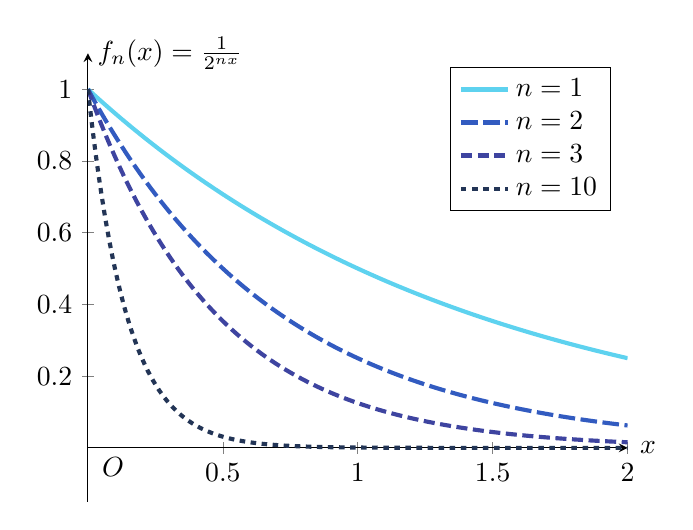
\begin{tikzpicture}
    \begin{axis}[
        axis lines = middle,
        xlabel = \(x\),
        ylabel = {\(f_n(x) = \frac{1}{2^{nx}}\)},
        xmin = 0, xmax = 2,
        ymin = -0.15, ymax = 1.1,
        xtick = {0,0.5,1,1.5,2},
        ytick = {0,0.2,0.4,0.6,0.8,1.0},
        legend style = {cells={anchor=west}, legend pos=north east},
        xlabel style={at={(ticklabel* cs:1.0)}, anchor=west, xshift=1pt},
        ylabel style={at={(ticklabel* cs:1.0)}, anchor=west, yshift=0pt},
        every axis plot/.append style={line width=3pt}
        ]
        \node[below left] at (axis cs:0.17,0) {$O$};
        % n = 1: f(x) = 1/(2^x)
        \addplot [
            domain=0:2,
            samples=200,
            thick,
            color={rgb,255:red,94; green,210; blue,239},
            line width=1.5pt
        ] {1/(2^x)};
        \addlegendentry{\(n=1\)}

        % n = 2: f(x) = 1/(2^{2x}) = 1/(4^x)
        \addplot [
            domain=0:2,
            samples=200,
            thick,
            color={rgb,255:red,50; green,91; blue,192},
            dash pattern=on 6pt off 2pt,
            line width=1.5pt
        ] {1/(4^x)};
        \addlegendentry{\(n=2\)}

        % n = 3: f(x) = 1/(2^{3x}) = 1/(8^x)
        \addplot [
            domain=0:2,
            samples=200,
            thick,
            color={rgb,255:red,62; green,68; blue,160},
            dash pattern=on 4pt off 2pt,
            line width=1.5pt
        ] {1/(8^x)};
        \addlegendentry{\(n=3\)}

        % n = 10: f(x) = 1/(2^{10x}) = 1/(1024^x)
        \addplot [
            domain=0:2,
            samples=200,
            thick,
            color={rgb,255:red,35; green,53; blue,86},
            dash pattern=on 2pt off 2pt,
            line width=1.5pt
        ] {1/(1024^x)};
        \addlegendentry{\(n=10\)}
    \end{axis}
    \end{tikzpicture}}
    \centeredcaption{图1：$f_n(x) = \frac{1}{2^{nx}} \to f(x) = 0$}{$\mathop{sup}\limits_{x\in X}\{ |f_n(x) - f(x)| \} = 1$}
    \end{minipage}
    \hfill
    %second fig
    \begin{minipage}[t]{0.48\textwidth}
    \centering
    \resizebox{0.9\textwidth}{!}{% 缩放以适应宽度
    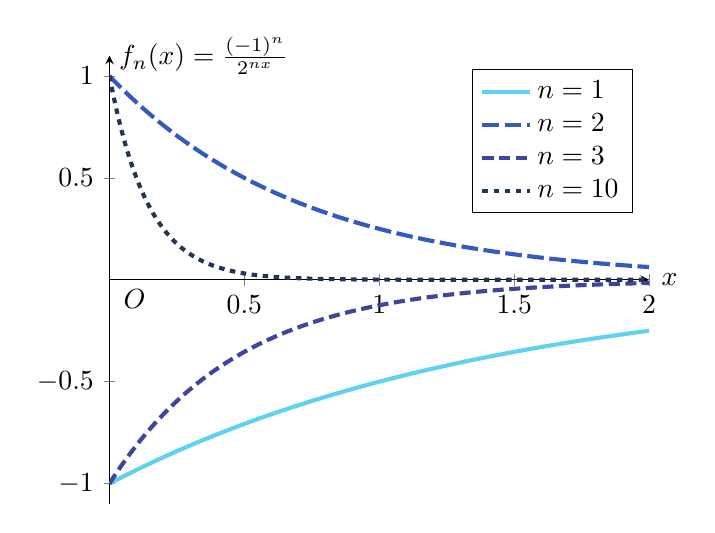
\begin{tikzpicture}
    \begin{axis}[
        axis lines = middle,
        xlabel = \(x\),
        ylabel = {\(f_n(x) = \frac{(-1)^n}{2^{nx}}\)},
        xmin = 0, xmax = 2,
        ymin = -1.1, ymax = 1.1,
        xtick = {0,0.5,1,1.5,2},
        ytick = {-1.0,-0.5,0,0.5,1.0},
        legend style = {cells={anchor=west}, legend pos=north east},
        xlabel style={at={(ticklabel* cs:1.0)}, anchor=west, xshift=1pt},
        ylabel style={at={(ticklabel* cs:1.0)}, anchor=west, yshift=0pt},
        every axis plot/.append style={line width=3pt}
        ]
        \node[below left] at (axis cs:0.17,0) {$O$};
        % n = 1: f(x) = 1/(2^x)
        \addplot [
            domain=0:2,
            samples=200,
            thick,
            color={rgb,255:red,94; green,210; blue,239},
            line width=1.5pt
        ] {-1/(2^x)};
        \addlegendentry{\(n=1\)}

        % n = 2: f(x) = 1/(2^{2x}) = 1/(4^x)
        \addplot [
            domain=0:2,
            samples=200,
            thick,
            color={rgb,255:red,50; green,91; blue,192},
            dash pattern=on 6pt off 2pt,
            line width=1.5pt
        ] {1/(4^x)};
        \addlegendentry{\(n=2\)}

        % n = 3: f(x) = 1/(2^{3x}) = 1/(8^x)
        \addplot [
            domain=0:2,
            samples=200,
            thick,
            color={rgb,255:red,62; green,68; blue,160},
            dash pattern=on 4pt off 2pt,
            line width=1.5pt
        ] {-1/(8^x)};
        \addlegendentry{\(n=3\)}

        % n = 10: f(x) = 1/(2^{10x}) = 1/(1024^x)
        \addplot [
            domain=0:2,
            samples=200,
            thick,
            color={rgb,255:red,35; green,53; blue,86},
            dash pattern=on 2pt off 2pt,
            line width=1.5pt
        ] {1/(1024^x)};
        \addlegendentry{\(n=10\)}
    \end{axis}
    \end{tikzpicture}}
    \centeredcaption{图2：$f_n(x) = \frac{(-1)^n}{2^{nx}} \to f(x) = 0$}{$\mathop{sup}\limits_{x\in X}\{ |f_n(x) - f(x)| \} = 1$}
    \end{minipage}

    % first fig
    \begin{minipage}[t]{0.48\textwidth}
    \centering
    \resizebox{0.9\textwidth}{!}{% 缩放以适应宽度
    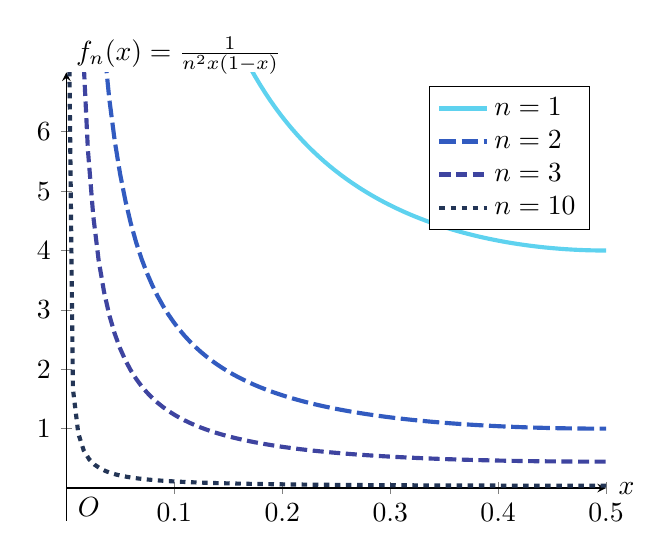
\begin{tikzpicture}
    \begin{axis}[
        axis lines = middle,
        xlabel = \(x\),
        ylabel = {\(f_n(x) = \frac{1}{n^2 x(1-x)}\)},
        xmin = 0, xmax = 0.5,
        ymin = -0.55, ymax = 7,
        xtick = {0,0.1,0.2,0.3,0.4,0.5},
        ytick = {0,1,2,3,4,5,6},
        legend style = {cells={anchor=west}, legend pos=north east},
        xlabel style={at={(ticklabel* cs:1.0)}, anchor=west, xshift=1pt},
        ylabel style={at={(ticklabel* cs:1.0)}, anchor=west, yshift=6pt},
        every axis plot/.append style={line width=3pt}
        ]
        \node[below left] at (axis cs:0.04,0) {$O$};
        % n = 1: f(x) = 1/(2^x)
        \addplot [
            domain=0:0.99,
            samples=200,
            thick,
            color={rgb,255:red,94; green,210; blue,239},
            line width=1.5pt
        ] {1/(x*(1-x))};
        \addlegendentry{\(n=1\)}

        % n = 2: f(x) = 1/(2^{2x}) = 1/(4^x)
        \addplot [
            domain=0:0.99,
            samples=200,
            thick,
            color={rgb,255:red,50; green,91; blue,192},
            dash pattern=on 6pt off 2pt,
            line width=1.5pt
        ] {1/(4*x*(1-x))};
        \addlegendentry{\(n=2\)}

        % n = 3: f(x) = 1/(2^{3x}) = 1/(8^x)
        \addplot [
            domain=0:0.99,
            samples=200,
            thick,
            color={rgb,255:red,62; green,68; blue,160},
            dash pattern=on 4pt off 2pt,
            line width=1.5pt
        ] {1/(9*x*(1-x))};
        \addlegendentry{\(n=3\)}

        % n = 10: f(x) = 1/(2^{10x}) = 1/(1024^x)
        \addplot [
            domain=0.001:0.9999,
            samples=200,
            thick,
            color={rgb,255:red,35; green,53; blue,86},
            dash pattern=on 2pt off 2pt,
            line width=1.5pt
        ] {1/(100*x*(1-x))};
        \addlegendentry{\(n=10\)}

    \end{axis}
    \end{tikzpicture}}
    \centeredcaption{图3：$f_n(x) = \frac{1}{n^2 x(1-x)} \to f(x) = 0$}{$\mathop{sup}\limits_{x\in X}\{ |f_n(x) - f(x)| \} = +\infty$}
    \end{minipage}
    \hfill
    %second fig
    \begin{minipage}[t]{0.5\textwidth}
    \centering
    \resizebox{0.9\textwidth}{!}{% 缩放以适应宽度
    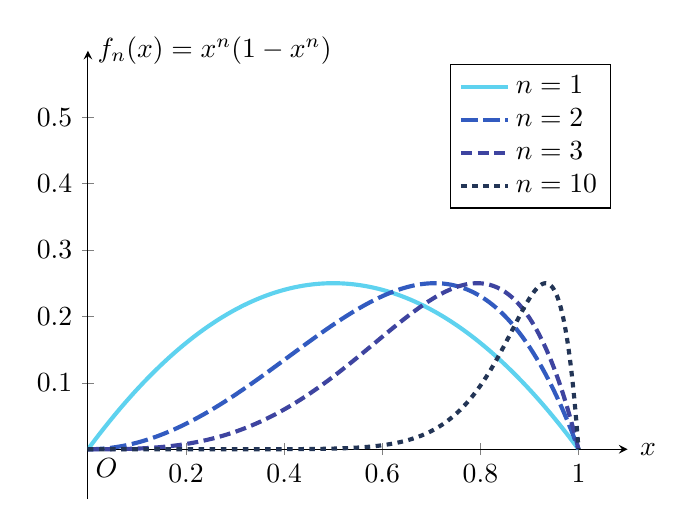
\begin{tikzpicture}
    \begin{axis}[
        axis lines = middle,
        xlabel = \(x\),
        ylabel = {\(f_n(x) = x^n(1-x^n) \)},
        xmin = 0, xmax = 1.1,
        ymin = -0.075, ymax = 0.6,
        xtick = {0,0.2,0.4,0.6,0.8,1},
        ytick = {0,0.1,0.2,0.3,0.4,0.5},
        legend style = {cells={anchor=west}, legend pos=north east},
        xlabel style={at={(ticklabel* cs:1.0)}, anchor=west, xshift=1pt},
        ylabel style={at={(ticklabel* cs:1.0)}, anchor=west, yshift=0pt},
        every axis plot/.append style={line width=3pt}
        ]
        \node[below left] at (axis cs:0.08,0) {$O$};
        % n = 1: f(x) = 1/(2^x)
        \addplot [
            domain=0:1,
            samples=200,
            thick,
            color={rgb,255:red,94; green,210; blue,239},
            line width=1.5pt
        ] {x*(1-x)};
        \addlegendentry{\(n=1\)}

        % n = 2: f(x) = 1/(2^{2x}) = 1/(4^x)
        \addplot [
            domain=0:1,
            samples=200,
            thick,
            color={rgb,255:red,50; green,91; blue,192},
            dash pattern=on 6pt off 2pt,
            line width=1.5pt
        ] {x^2*(1-x^2)};
        \addlegendentry{\(n=2\)}

        % n = 3: f(x) = 1/(2^{3x}) = 1/(8^x)
        \addplot [
            domain=0:1,
            samples=200,
            thick,
            color={rgb,255:red,62; green,68; blue,160},
            dash pattern=on 4pt off 2pt,
            line width=1.5pt
        ] {x^3*(1-x^3)};
        \addlegendentry{\(n=3\)}

        % n = 10: f(x) = 1/(2^{10x}) = 1/(1024^x)
        \addplot [
            domain=0:1,
            samples=500,
            thick,
            color={rgb,255:red,35; green,53; blue,86},
            dash pattern=on 2pt off 2pt,
            line width=1.5pt
        ] {x^10*(1-x^10)};
        \addlegendentry{\(n=10\)}

    \end{axis}
    \end{tikzpicture}}
    \centeredcaption{图4：$f_n(x) = x^n(1-x^n) \to f(x) = 0 \vphantom{\dfrac{1}{1}}$ }{$\mathop{sup}\limits_{x\in X}\{ |f_n(x) - f(x)| \} = 1/4$}
    \end{minipage}
\end{figure} \vspace{1em}

第四例的情况则有所不同：\vspace{0.5em}

(4)~$f_n(x) = x^n (1-x^n),~X = [0,1]$.
$\{ f_n (x)\} $在$X$上逐点收敛于常函数$f(x) = 0$，但不是一致收敛.
注意在边界点$x_0 = 0$和$x_0 = 1$处$f_n(x_0)$都恒为$0$，
这个函数列的“不稳定因素”出现在定义域内部.
观察$\{ f_n(x) \}$的图像，
发现它随着$n$增大像波浪一样向右推进，
且波峰永远保持在$y = \frac{1}{4}$的高度而不落下.
这是不一致收敛的直接原因.
如用命题3，只需要用$\{ x_n \}$来追踪波峰的位置，
即：取$x_n$为$|f_n(x) - f(x)|$的最大值点即可.
这实际上也是对定义的直接验证.

\subsubsection{函数项级数一致收敛的判别法}

函数项级数收敛等同于部分和序列收敛，
因此也可以更细致地谈论\textbf{函数项级数的逐点收敛}（即部分和序列逐点收敛）
或\textbf{一致收敛}（即部分和序列一致收敛）.
不过，一般情况下无法计算出部分和序列的具体表达式，
我们很难直接判断一致收敛性.
仅有柯西准则和三条判别法供我们使用：\vspace{1em}

\textbf{1.~~函数项级数一致收敛的柯西收敛原理}~~\textit{函数项级数$\sum_{n=1}^{\infty} u_n(x)$ 在定义域$X$上一致收敛的充要条件是：
对于任意给定的 \(\epsilon > 0\)，存在一个只依赖于 \(\epsilon\) 的 \( N\)，使得对任意的 \( n > N \) 及任意正整数 \( p \)，不等式：
\[ \left| \sum_{k=n+1}^{n+p} u_k(x) \right| < \epsilon \]
对于一切 \( x \in X \) 成立.} \vspace{1.25em}

函数项级数一致收敛的柯西收敛原理也可以作为定义使用，
但是作为判别法则不太好用.
在数项级数部分，曾经提及了柯西收敛原理的一些用法，
在证明函数项级数（不）一致收敛时也可以使用.
不过，首选仍然是下面三个判别法.\vspace{1.25em}

\textbf{2.~~强级数判别法}~~\textit{若函数项级数$\sum_{n=1}^{\infty} u_n(x)$的一般项满足：
$|u_n(x)| \leq1 a_n, \quad \forall x \in X $ ，
且正项级数 $ \sum_{n=1}^{\infty} a_n $ 收敛，
则该函数项级数在$X$上一致收敛.} \vspace{0.75em}

这里，$a_n$可以视为将$u_n(x)$放大为常函数.
注意这个定理并非充要条件，
即如果级数$\ss a_n$不收敛，
不能推出函数项级数$\ss u_n(x)$不一致收敛，
\textbf{即便把$a_n$取为$|u_n(x)|$的上确界（最大值）也是如此.}
这个判别法一般用在$\{ u_n (x)\}$是非负函数列时
（这与数项级数要先区分正项级数和一般项级数类似）.
若$\{ u_n(x) \}$不是非负函数列，
这个定理是相当弱的，
用处不大.
下面两个判别法用来针对$\{ u_n(x) \}$不是非负函数列的情况：\vspace{1.25em}

\textbf{3.~~狄利克雷判别法}~~\textit{设函数序列$\{a_n (x)\}$和$\{ b_n (x)\}$在$X$上有定义，
且各自满足下列条件：}

\textit{(1)~在 \( X \) 中任意取定一个 \( x \)，数列 \(\{a_n(x)\}\) 对 \( n \) 单调，且函数序列 \(\{a_n(x)\}\) 在 \( X \) 上一致收敛于0；}

\textit{(2)~函数项级数 $\sum_{n=1}^{\infty} b_n(x) $的部分和序列 \(\{B_n(x)\}\) 在 \( X \) 上一致有界，}

\textit{则函数项级数 $\sum_{n=1}^{\infty} a_n(x)b_n(x)$ 在 \( X \) 上一致收敛.} \vspace{1em}

\textbf{4.~~阿贝尔判别法}~~\textit{设函数序列$\{a_n (x)\}$和$\{ b_n (x)\}$在$X$上有定义，
且各自满足下列条件：}

\textit{(1)~在 \( X \) 中任意取定一个 \( x \)，数列 \(\{a_n(x)\}\) 对 \( n \) 单调，且函数序列 \(\{a_n(x)\}\) 在 \( X \) 上一致有界；}

\textit{(2)~函数项级数 $\sum_{n=1}^{\infty} b_n(x) $在 \( X \) 上一致收敛，}

\textit{则函数项级数 $\sum_{n=1}^{\infty} a_n(x)b_n(x)$ 在 \( X \) 上一致收敛.} \vspace{1.5em}

这两个判别法的记忆和使用与数项级数中完全类似，
只需要把定理中的“收敛”都改为“一致收敛”，
有界都改为“一致有界”.
另外注意“单调”是指对$n$单调（和数列的单调类似），
而不是指函数$a_n(x)$是单调函数.
为了避免歧义，也可以称之为\textbf{渐升}或者\textbf{渐降}函数列.

~\par

\subsubsection{函数项级数一致收敛的性质}

我们的最终目的是研究函数项级数的和函数$S(x)$的性质，
包括连续性、可积性和可微性.
有这些性质，同时也意味着可逐项求极限、求积分和求导.
其中，连续性/可积性的前提条件是$u_n(x)$连续/可积，且\textbf{函数项级数在区间内一致收敛}，
而可微性的前提条件是$u_n(x)$连续可导，且\textbf{逐项求导后的函数项级数在区间内一致收敛}.\vspace{1em}

\textbf{定理（连续性，逐项求极限）}~~\textit{设函数项级数 $\displaystyle\sum_{n=1}^{\infty} u_n(x)$ 在闭区间 $[a,b]$ 上一致收敛，
且每一项 $u_n(x)$ $(n=1,2,\dots)$ 都在 $[a,b]$ 上连续，
则其和函数$S(x)$在 $[a,b]$ 上也连续.且函数项级数可以逐项求极限，即：}
\begin{eq1}
    \lim\limits_{x \to x_0} \ss u_n(x) = \ss \lim\limits_{x \to x_0} u_n(x)
\end{eq1}\vspace{0.25em}

该定理也可逆用来判定函数项级数不一致收敛：
如果各个$u_n(x)$在$[a,b]$上都连续，
而$S(x)$却不连续，
就说明$\ss u_n(x)$在$[a,b]$上不一致收敛.\vspace{1.25em}

\textbf{定理（可积性，逐项求积分）}~~\textit{若级数 $\displaystyle\sum_{n=1}^{\infty} u_n(x)$ 在闭区间 $[a,b]$ 上一致收敛，
且每一项 $u_n(x)\ (n=1,2,\dots)$ 都在 $[a,b]$ 上连续，
则其和函数$S(x)$在 $[a,b]$ 上可积，且可逐项积分，即：}
\[
\int_a^b S(x)\,dx=\sum_{n=1}^{\infty}\int_a^b u_n(x)\,dx.
\]

\textbf{定理（可微性，逐项求导）}~~
\textit{设函数项级数 $\displaystyle\sum_{n=1}^{\infty} u_n(x)$ 在闭区间 $[a,b]$ 上点点收敛，
且满足：（1）每一项 $u_n(x)$ 的导函数 $u_n'(x)$ 在 $[a,b]$ 上连续；
（2）级数 $\displaystyle\sum_{n=1}^{\infty} u_n'(x)$ 在 $[a,b]$ 上一致收敛.
则其和函数$S(x)$在 $[a,b]$ 上连续可导，且可逐项求导，即：}
\begin{eq1}
S'(x)=\sum_{n=1}^{\infty} u_n'(x)
\end{eq1}\vspace{0.5em}

以上三条定理中的“闭区间$[a,b]$”均可改为区间，包括闭区间、开区间和半开半闭区间.

在题目中，有时需要用逐项求积分/求导的技巧来计算和函数$S(x)$.
除了计算出结果之外，
验证定理成立的条件（尤其是一致收敛性）也是关键的步骤.

有时会遇到这样的情况：解题明显要使用逐项求积分/求导，
但是在定义区间上却并不满足一致收敛性.
这时该怎么办？
根据我们此前的讨论（10.2.2），
不一致收敛往往是因为区间端点的行为异常，
即使区间端点并不包括在区间内.
10.2.2中的例(1)(2)(3)的$x=0$都是如此.
只要把$0$的任意邻域从定义域$X$中挖去，
即取区间左端点为任意小的正数$\epsilon$，
都能让函数项级数一致收敛.
这种排除边界效应而达到的一致收敛性称为\textbf{内闭一致收敛}.
即：在定义域的任意子闭区间内一致收敛.
当函数项级数（或逐项求导后的级数）满足内闭一致收敛时，
意味着它可以在定义域的任意子闭区间内逐项求积分（逐项求导）.
这其实就够用了.
对开区间定义域而言，
其中的任何一点都能被包含在定义域的某个子闭区间内，
从而可以通过逐项求积分（逐项求导）求出和函数的取值.
这无疑是一种赖皮且好用的策略.

\subsubsection{幂级数的性质}

解决一道典型的幂级数求和问题，需要依次解决以下的问题：

(1)~计算收敛域；
(2)~判断一致收敛性（内闭一致收敛性）；
(3)~判断连续性、可积性和可微性，以及逐项求积分/求导后的收敛域；
(4)~利用已知的幂级数求和结果（泰勒级数）.
本节的知识点就是围绕这些方面展开.\vspace{1em}

\textbf{1.~~收敛半径、收敛域、收敛区间}\vspace{0.5em}

幂级数$\sum_{n=0}^{\infty} a_n (x-x_0)^n$的收敛域是以$x_0$为中心的区间，
区间左右端点距中心的距离相等，
该距离称为\textbf{收敛半径}$R$.
另外，把开区间$(x_0 - R, x_0+R)$称为\textbf{收敛区间}.
注意收敛域不一定等于收敛区间.
当$R$为有限数时，
收敛域可能是$(x_0 - R, x_0+R),[x_0 - R, x_0+R),(x_0 - R, x_0+R],[x_0 - R, x_0+R]$.
因此，求幂级数的收敛域有两个步骤：
(1)~求收敛半径（得到收敛区间）；
(2)~单独判断左右端点处幂级数是否收敛.

求幂级数的收敛半径一般用如下定理：\vspace{1em}

\textbf{定理}~~
\textit{设幂级数$\sum_{n=0}^{\infty} a_n x^n$满足：}
$\lim_{n\to\infty}\left|\frac{a_{n+1}}{a_n}\right|=l$.
\textit{则该级数的收敛半径 $R$ 满足：}

\textit{（1）若 $0<l<+\infty$，则 $R=\dfrac{1}{l}$；}

\textit{（2）若 $l=0$，则 $R=+\infty$；}

\textit{（3）若 $l=+\infty$，则 $R=0$.}\vspace{1em}

如果该定理不适用，
不代表收敛半径不存在.
须知该定理是由达朗贝尔判别法推出的.
因此特殊情况下需要回归拉朗贝尔判别法来求收敛半径.
例如：$\ss (-1)^{n-1}\frac{2n+1}{n}x^{2n}$.\vspace{1em}

\textbf{2.~~一致收敛性}\vspace{0.25em}

一句话：\textbf{幂级数在收敛域内是内闭一致收敛的}.
即幂级数在收敛域的任意子闭区间上一致收敛.
同时也意味着，
如果收敛域是（单侧）闭区间，
那么可以直接说幂级数在收敛域上（单侧）一致收敛.\vspace{1em}

\textbf{3.~连续性、可积性、可微性}\vspace{0.25em}

幂级数的收敛域若为闭区间，
由一致收敛性，
可以直接推知\textbf{和函数在闭区间上连续}.
值得注意的是收敛域为开区间的情况.
即使幂级数在开区间上不一定一致收敛，
我们也可以推出\textbf{和函数在开区间上连续}.
奥妙就在于幂级数的内闭一致收敛性.
因为幂级数在收敛域的任意子闭区间内一致收敛，
则和函数就在收敛域的任意子闭区间内连续.
这种性质或可称为“内闭连续性”.
但稍加思考便会发现，
开区间上的所谓“内闭连续性”其实就等于说开区间上连续.

综上，\textbf{幂级数的和函数在收敛域内连续（不论收敛域是开是闭）.}

同样的道理，还可以知道，\textbf{幂级数在收敛域内总是可以逐项求积分}.

逐项求导的情况有所不同.
逐项求导定理要求的是逐项求导后的级数一致收敛.
由幂级数的内闭一致收敛性，
我们可以推出幂级数在收敛域的任意子闭区间内可逐项求导，
这即是说\textbf{幂级数在收敛区间内可逐项求导}.
但是，即使原本的幂级数在收敛区间内（单侧）一致收敛，
逐项求导后的级数也不一定在收敛区间内（单侧）一致收敛.
因此，\textbf{收敛域的（闭区间）端点处不一定可以逐项求导}.
例如：$\ss (-1)^{n-1} \frac{x^n}{n}$的收敛域是$(-1,1]$，
而逐项求导后的级数$\sum_{n=0}^{+\infty} (-1)^n x^n$收敛域是$(-1,1)$，
且在收敛域内不是一致收敛.
在做题时需要格外小心这一点.

根据上述整理，
我们知道幂级数逐项求积分或求导后，
收敛半径不会缩小.
那么收敛半径会增大吗？
考虑对任意一个幂级数逐项求积分之后又逐项求导，
结果还是原来的幂级数，
收敛半径自然也不变.
已知这两步操作都不会使收敛半径减小，
那么为了维持收敛半径不变，
这两步操作也都不可能使收敛半径增大.
最终结论是：
\textbf{幂级数逐项求积分或求导数后，收敛半径不变.} \vspace{1em}

\textbf{4.~泰勒级数}\vspace{0.25em}

我们曾经学习过泰勒公式：
\begin{eq1}
    f(x) =  f(x_0) + \frac{f'(x_0)}{1!}(x-x_0) + \frac{f''(x_0)}{2!}(x-x_0)^2 + \cdots + \frac{f^{(n)}(x_0)}{n!}(x-x_0)^n + R_n(x)
\end{eq1}

其中，$R_n(x)$是余项.
当时我们强调，
当$R_n(x)$为拉格朗日余项时，
可以用来估计泰勒多项式近似$f(x)$的误差.
当$x$充分接近$x_0$时，
$R_n(x)$可以充分小.
这是基于$n$有限的情况做出的讨论.
而当$n \to \infty$时，
泰勒多项式的项数趋于无穷，
可以看成一个幂级数，
称为$f(x)$的\textbf{泰勒级数}：
$$
f(x) \sim \sum_{n=0}^{\infty} \frac{f^{(n)}(x_0)}{n!}(x-x_0)^n
$$

$f(x)$能写出泰勒级数的前提条件是$f(x)$无穷阶可导.
上面的公式之所以用$\sim$连接而不写等号，
是因为泰勒级数不一定收敛到$f(x)$——
至少，不一定在$\mathbb{R}$上处处收敛到$f(x)$.
显然，$f(x)$的泰勒级数在$x$处收敛到$f(x)$的充要条件是
$R_n(x) \to 0$.
但即使取$R_n(x)$为拉格朗日余项，
也难以计算何时$R_n(x) \to 0$.
有同学可能想：
这不就是求泰勒级数的收敛域吗，
何必这么麻烦要借助余项呢？
这样想是不对的.
因为$f(x)$的泰勒级数即使收敛，
也不一定收敛到$f(x)$.
有经典反例：\vspace{0.25em}
\begin{eq1}
    \setstretch{1.25}
    f(x) =
    \begin{cases}
        e^{-1/x^2} &\quad x \ne 0 \\
        0 &\quad x = 0
    \end{cases}
\end{eq1}

\setstretch{1.75}

该函数的泰勒级数$0 + \frac{0}{1!}x + \frac{0}{2!}x^2 + \cdots + \frac{0}{n!}x^n$显然在$\mathbb{R}$上收敛到$0$.
这说明$f(x)$的泰勒级数只有在$x=0$处收敛到$f(x)$.
可见，泰勒级数展开（或称幂级数展开）的范围与泰勒级数的收敛域不是一回事.

以下初等函数的泰勒展开是很重要的.
要计算一般的幂级数的和函数，
需要依赖这些已知的幂级数求和结果.
除了泰勒级数本身（在第四章已经要求背过），
还必须记住相应$x$的范围.
\begin{eq1}
    e^x &= 1 + x +\frac{x^2}{2!} + \cdots +\frac{x^n}{n!} + \cdots, \quad x \in (-\infty, +\infty) \\[5pt]
    \sin x &= x - \frac{x^3}{3!} + \frac{x^5}{5!} + \cdots + (-1)^{k}\frac{x^{2k+1}}{(2k+1)!} +\cdots, \quad x \in (-\infty, +\infty) \\[5pt]
    \cos x &= 1 -\frac{x^2}{2!} + \frac{x^4}{4!} +\cdots + (-1)^{k} \frac{x^{2k}}{2k!} +\cdots, \quad x \in (-\infty, +\infty) \\[5pt]
    \arctan x &= x - \frac{x^3}{3} + \frac{x^5}{5} + \cdots + (-1)^n \frac{x^{2n+1}}{2n+1} +\cdots, \quad x \in [-1,1] \\[5pt]
    \ln (1+x) &= x - \frac{x^2}{2} + \frac{x^3}{3} - \cdots +(-1)^{n-1} \frac{x^n}{n} +\cdots, \quad x \in (-1,1] \\[5pt]
    (1+x)^a &= 1 + ax + \frac{a(a-1)}{2!}x^2 + \cdots + \frac{a(a-1)\cdots (a-n+1)}{n!}x^n +\cdots, \quad x \in (-1,1) \\[5pt]
\end{eq1}

\subsection{解题技巧}

\subsubsection{判断级数收敛性}

判断级数收敛性的基本步骤如下.
首先判断是级数是否是正项级数. 如果是，用正项级数的判别法.
如果不是，需考虑绝对收敛和条件收敛.
对于绝对收敛性的判别，只需要给级数加绝对值，然后回归正项级数的判别法.
对于条件收敛性的判别，只需要思考使用莱布尼茨判别法、狄利克雷判别法还是阿贝尔判别法即可.

要点：注意各个判别法的使用条件，尤其注意不要对一般项级数使用正项级数的判别法（如比较判别法）.
背诵清楚狄利克雷判别法和阿贝尔判别法的条件.
如果发现各个判别法都没有用，可以考虑更细致的估阶方法（如下一小节讲的泰勒展开）.

\begin{example}[2023]
\label{ex:ch10-01}
判断下列级数敛散性:

(1)~~
$\sum_{n=3}^{\infty} \frac{2}{n \ln \sqrt{n}}$

(2)~~
$\sum_{n=1}^{\infty} \frac{3 \sqrt[5]{n} + 1}{(\sqrt[4]{n}+ n)(\sqrt[3]{n} + n)}$

(3)~~
$\sum_{n=1}^{\infty} \left( \frac{4 \cdot 3^n}{5^n} - \frac{1}{n} + \frac{1}{n+2} \right)$
\end{example}

\begin{solution}
(1)~~由对数性质知级数通项$a_n = \frac{4}{n \ln n}$.
    证明该级数的发散性是课本例题.
    由无穷积分判别法可知，该级数的敛散性等价于相应无穷积分的敛散性：
    \begin{eq1}
        \int_{3}^{+\infty} \frac{1}{x \ln x}~\d x
    \end{eq1}

    用凑微分法计算该无穷积分：
    \begin{eq1}
        \int_{3}^{+\infty} \frac{1}{x \ln x}~\d x
        &= \int_{3}^{+\infty} \frac{1}{\ln x}~\d (\ln x) \\
        &= \ln \ln x \bigg|_{3}^{+\infty} \\
        &= \lim\limits_{x \to + \infty} \ln \ln x - \ln \ln 3
    \end{eq1}

    式中的极限显然是发散的，即无穷积分是发散的. 因此原级数发散，

    (2)~~当$n \to +\infty$时，级数通项有以下的无穷小量等价关系：
    \begin{eq1}
        \sum_{n=1}^{\infty} \frac{3 \sqrt[5]{n} + 1}{(\sqrt[4]{n}+ n)(\sqrt[3]{n} + n)}
        \sim
        \frac{3 \sqrt[5]{n}}{n \cdot n} \sim \frac{3}{n^{9/5}}
    \end{eq1}

    由$p$级数的结论可知$\sum_{n=1}^{\infty} \frac{3}{n^{9/5}}$收敛，因而原级数收敛.

    (3)~~部分合并级数通项：
    \begin{eq1}
        a_n = \frac{4 \cdot 3^n}{5^n} - \frac{1}{n} + \frac{1}{n+2}
        = \frac{4 \cdot 3^n}{5^n} - \frac{2}{n(n+2)}
    \end{eq1}

    我们发现级数$\sum_{n=1}^{\infty} \frac{4 \cdot 3^n}{5^n}$是$|q|<1$的等比级数，因此收敛；
    而级数$\sum_{n=1}^{\infty} \frac{-2}{n(n+2)}$的通项等价于$\frac{-2}{n^2}$，由$p$级数的结论可知收敛.
    因此：
    \begin{eq1}
        \sum_{n=1}^{\infty} a_n = \sum_{n=1}^{\infty} \frac{4 \cdot 3^n}{5^n} + \sum_{n=1}^{\infty} \frac{-2}{n(n+2)}
    \end{eq1}
    是收敛的.
\end{solution}

\begin{example}
\label{ex:ch10-02}
设$p$和$q$都是正实数. 讨论级数$\sum_{n=2}^{\infty} \frac{1}{n^p \ln^q n}$的敛散性.
\end{example}

\begin{analysis}
当$n \to \infty$时，$\ln n \ll n$.
    因此可以用比较判别法说明这个级数的收敛性基本和$p$级数类似.
    但是这个方法对于$p=1$失效.
    不过好在此时回归了可以用无穷积分判别法的经典情形.
\end{analysis}

\begin{solution}
i)~当$p > 1$时，级数通项可以放大：$\frac{1}{n^p \ln^q n} < \frac{1}{n^p}$.
    而$p$级数$\sum_{n=2}^{\infty} \frac{1}{n^p}$收敛，由比较判别法可知原级数收敛.

    ii)~当$p < 1$时，我们通过$p$级数的结论和$\ln n$增长较慢的事实，猜测级数是发散的.
    因此只需与$\frac{1}{n}$比较：
    \begin{eq1}
        \limn \frac{1/(n^p \ln^q n)}{1/n} = \limn \frac{n^{1-p}}{\ln^q n} = +\infty
    \end{eq1}
    而级数$\ss \frac{1}{n}$是发散的.
    由比较判别法可知原级数发散.

    iii)~当$p = 1$时，由无穷积分判别法可知，该级数的敛散性等价于相应无穷积分的敛散性：
    \begin{eq1}
        \int_{2}^{+\infty} \frac{1}{x \ln^q x}~\d x
    \end{eq1}

    计算如下：
    \begin{eq1}
        \int_{2}^{+\infty} \frac{1}{x \ln^q x}~\d x
        &= \int_{2}^{+\infty} \frac{1}{\ln^q x}~ \d (\ln x) \\[4pt]
        &=
        \begin{cases}
            \ln \ln x \bigg|_{2}^{+\infty} = \lim\limits_{x \to +\infty} \ln \ln x - \ln \ln 2 ~~(q=1)\\[4pt]
            \frac{(\ln x)^{-q+1}}{-q+1} \bigg|_{2}^{+\infty} = \lim\limits_{x \to +\infty} \frac{(\ln x)^{-q+1}}{-q+1} - \frac{(\ln 2)^{-q+1}}{-q+1} ~~(q \ne 1)
        \end{cases}
    \end{eq1}

    可见，当$q > 1$时，无穷积分收敛；当$0 < q \le 1$时，无穷积分发散.

    综上，当$0<p<1$，或$p =1$且$0 < q \le 1$时，级数发散；
    当$p>1$，或$p=1$且$q > 1$时，级数收敛.
\end{solution}

\begin{example}
\label{ex:ch10-03}
判断级数$\sum_{n=2}^{\infty} \frac{1}{(\ln n)^{\ln n}}$的敛散性.
\end{example}

\begin{analysis}
问题的实质是分析$(\ln n)^{\ln n}$的增长速率，看是否快于$n^{1+\epsilon}$.
\end{analysis}

\begin{solution}
对级数通项做如下变形：
    \begin{eq1}
        a_n = \frac{1}{(\ln n)^{\ln n}} = \frac{1}{e^{\ln \ln n \cdot \ln n} } = \frac{1}{n^{\ln \ln n}}
    \end{eq1}

    显然当$n$充分大时，有$\ln \ln n > 2$，从而$\frac{1}{n^{\ln \ln n}} < \frac{1}{n^2}$.
    因为级数$\sum_{n=1}^{\infty} \frac{1}{n^2}$收敛，由比较判别法可知原级数收敛.
\end{solution}

\begin{example}
\label{ex:ch10-04}
判断级数$\ss \left( \frac{1}{n} - \sin \frac{1}{n} \right)$的敛散性.
\end{example}

\begin{analysis}
{第一章中求极限方法可以放在正项级数的背景下考察.}
\end{analysis}

\begin{solution}
当$n \to \infty$时，$x = \frac{1}{n} \to 0$是无穷小量.
    容易证明$x - \sin x \sim \frac{x^3}{6}~(x \to 0)$，
    即$\frac{1}{n} - \sin \frac{1}{n}$与$\frac{1}{n^3}$是同阶无穷小量.
    而级数$\ss \frac{1}{n^3}$收敛.
    由比较判别法可知原级数收敛.
\end{solution}

\begin{example}
\label{ex:ch10-05}
设$a_n = \cos n \pi \cdot \ln \left( 1 + \frac{1}{\sqrt{n}} \right)$.

(1)~判断级数$\ss a_n$的收敛性（包括绝对收敛性）.

(2)~判断级数$\ss a_n^2$的收敛性.
\end{example}

\begin{solution}
(1)~~先判断绝对收敛性.
    当$n \to \infty$时，有如下的等价无穷小关系：
    \begin{eq1}
        |a_n| = \ln \left( 1+ \frac{1}{\sqrt{n}} \right) \sim \frac{1}{\sqrt{n}}
    \end{eq1}
    而级数$\ss \frac{1}{\sqrt{n}}$发散.
    由比较判别法可知，原级数不是绝对收敛.

    再判断级数$\ss a_n$的收敛性.
    注意到$\cos n \pi = (-1)^n$，该级数是交错级数.
    而$\ln \left( 1+ \frac{1}{\sqrt{n}} \right)$单调递减趋于$0$.
    故由莱布尼茨判别法可知，原级数发散.

    综上，级数$\ss a_n$条件收敛.

    (2)~~级数$\ss a_n^2$是正项级数.
    有如下的等价无穷小关系：
    \begin{eq1}
        a_n^2 = \ln^2 \left( 1+ \frac{1}{\sqrt{n}} \right) \sim \frac{1}{n}
    \end{eq1}
    而级数$\ss \frac{1}{n}$发散.
    由比较判别法可知，原级数发散.
\end{solution}

\begin{example}
\label{ex:ch10-06}
判断级数敛散性：$\ss \frac{\sin (2n)}{n+ \dfrac{1}{n}} \cdot \left( 1+ \frac{1}{n}\right)^n$.
\end{example}

\begin{analysis}
首先发现该级数不是正项级数，也不是交错级数，因此考虑用狄利克雷判别法或者阿贝尔判别法.
    观察级数中各项的特征.
    $\sin 2n$是典型的部分和有界的序列.
    而$\left( 1+\frac{1}{n} \right)^n$单调递增趋于$e$是熟知的结论.
    以这两点观察作为突破口.
\end{analysis}

\begin{solution}
当$n \to \infty$时，$\left( 1+\frac{1}{n} \right)^n$有界且单调递增（教材结论，可以不加证明直接使用）.
    由阿贝尔判别法，如果证明了级数$\ss \frac{\sin (2n)}{n+\dfrac{1}{n}}$收敛，就证明了原级数收敛.

    在级数$\ss \frac{\sin (2n)}{n+\dfrac{1}{n}}$中，
    $\sin (2n)$的部分和序列$\{ B_n \}$有界.
    事实上：
    \begin{eq1}
        B_n = \frac{1}{2\sin 1} \left( \sin (2n+1) - \sin 1 \right)
    \end{eq1}
    另一方面，序列$\left \{ \frac{1}{n + \frac{1}{n}}\right \}$显然单调趋于$0$.
    由狄利克雷判别法可知级数收敛.
\end{solution}

\subsubsection{*泰勒展开判断级数敛散性}

如果令$x = \frac{1}{n}$，则会发现$p$级数的通项其实是单项式$x^{p}$（单项式）.
也就是说，所有换元后具有单项式形式（$x \to 0$）的级数，我们都是知道敛散性的.
而我们又知道，任何$n$阶可导的函数都可以通过$n$阶泰勒展开，表示成多项式+余项的形式.
因此，在泰勒展开之后，只要保证余项构成的级数收敛，就能根据$p$级数的结论轻易判断原级数是否收敛.

这个方法对于一般项级数都是适用的，而且未必要把$\frac{1}{n}$看成$x$来展开，只要$n \to \infty$时$x \to 0$皆可.

\begin{example}
\label{ex:ch10-07}
判断级数敛散性：$\sum_{n=2}^{\infty} \frac{(-1)^n}{\sqrt{n} + (-1)^{n}}$
\end{example}

\begin{analysis}
该级数是交错级数，但是$\frac{1}{\sqrt{n} + (-1)^n}$不是单调递减的，故不能用莱布尼茨判别法.
    这里我们用泰勒展开强行解决.
\end{analysis}

\begin{solution}
对通项进行泰勒展开（$x = \frac{(-1)^n}{\sqrt{n}}$）：

    \begin{eq1}
        \frac{(-1)^n}{\sqrt{n} + (-1)^n}
        &= \frac{(-1)^n}{\sqrt{n}} \cdot \frac{1}{1 + \dfrac{(-1)^n}{\sqrt{n}}} \\
        &= \frac{(-1)^n}{\sqrt{n}} \cdot \left( 1 - \frac{(-1)^n}{\sqrt{n}} + \frac{1}{n} + o(\frac{1}{n}) \right) \\
        &= \boxed{\frac{(-1)^n}{\sqrt{n}}} - \boxed{\frac{1}{n}} + \boxed{\frac{(-1)^n}{n^{3/2} }+ o(\frac{1}{n^{3/2}})} \\[-6pt]
         & ~~~\text{条件收敛}~~\text{发散} ~~~~~~~~~\text{绝对收敛}
    \end{eq1}

如此，原级数的通项能被拆成三部分（用三个方框表示）之和.
每一部分构成的级数分别是条件收敛、发散和绝对收敛的.
它们相加所构成的级数是发散的.
\end{solution}

\begin{example}
\label{ex:ch10-08}
判断级数敛散性：$\sum_{n=2}^{\infty} \frac{(-1)^n}{\sqrt{n + (-1)^{n}}}$
\end{example}

\begin{solution}
对通项进行泰勒展开（$x = \frac{(-1)^n}{n}$）：
    \begin{eq1}
        \sum_{n=2}^{\infty} \frac{(-1)^n}{\sqrt{n + (-1)^{n}}}
    &= \frac{(-1)^n}{\sqrt{n}} \cdot \frac{1}{\sqrt{1 + \dfrac{(-1)^n}{n}}} \\
    &= \frac{(-1)^n}{\sqrt{n}} \cdot \left( 1 - \frac{1}{2} \cdot \frac{(-1)^n}{n} + o(\frac{1}{n}) \right) \\
    &= \boxed{\frac{(-1)^n}{\sqrt{n}}} - \boxed{\frac{1}{2} \cdot \frac{1}{n^{3/2}} + o(\frac{1}{n^{3/2}})} \\[-6pt]
    & ~~~\text{条件收敛}~~~~~~~~~~\text{绝对收敛}
    \end{eq1}

如此，原级数的通项能被拆成两部分（用两个方框表示）之和.
这两部分构成的级数分别是条件收敛和绝对收敛的.
它们相加所构成的级数是条件收敛的.
\end{solution}

结合上面两道例题，说明一下泰勒展开法的注意事项：

(1)~与泰勒展开法求极限类似的，需要注意展开的阶数.
只要保证余项是$o\left(\frac{1}{n^{1+\epsilon}}\right)$，
$\epsilon > 0$，那么余项就一定是绝对收敛的，无需再做更高阶的展开.
特别注意，当通项是$o \left(\frac{1}{n} \right)$时，不一定收敛（例如$\frac{1}{n \ln n}$）.
所以最好多展开一项.
例如上面两道例题中，都展开到了$\frac{1}{n^{3/2}}$的项.\vspace{0.5em}

(2)~最后判断敛散性时，用到了级数收敛性相加的性质，即从通项中剔除收敛的部分，不影响级数的收敛性.
这是教材定理，可以直接使用.
但事实上，还可以类似地判断出绝对收敛性.
例\ref{ex:ch10-08}就用到了以下的结论：\vspace{1em}

\textit{i)~~若$\ss a_n$与$\ss b_n$都绝对收敛，则$\ss \left( a_n + b_n \right)$绝对收敛.}

\textit{ii)~~若$\ss a_n$与$\ss b_n$一个绝对收敛，一个条件收敛，则$\ss \left( a_n + b_n \right)$条件收敛.}

\textit{iii)~~若$\ss a_n$与$\ss b_n$都条件收敛，则$\ss \left( a_n + b_n \right)$收敛，但不能确定是否绝对收敛.}\vspace{1.5em}

这些结论很简单，但是教材上没有直接提出.
因此在用的时候最好证明一下.

\begin{example}
\label{ex:ch10-09}
证明上面的结论.
\end{example}

\begin{proof}
已知每种情况下级数$\ss \left( a_n + b_n \right)$都收敛.
    这里只分析绝对收敛性.

    i)~~由三角不等式：$|a_n + b_n| \le |a_n| + |b_n|$.
    由级数$\ss a_n$和$\ss b_n$绝对收敛可知$\ss \left( |a_n| + |b_n| \right)$收敛，从而
    由比较判别法可知级数$\ss | a_n + b_n |$收敛.

    ii)~~不妨设$\ss a_n$绝对收敛，$\ss b_n$条件收敛. 用反证法.
    假设$\ss |a_n + b_n|$收敛.
    由三角不等式，$|b_n| = |\left( a_n + b_n \right) - a_n| \le |a_n + b_n| + |a_n|$.
    又由级数$\ss a_n$绝对收敛，可知级数$\ss \left( |a_n + b_n| + |a_n| \right)$收敛，
    从而由比较判别法可知级数$\ss |b_n|$收敛，矛盾.
    故级数$\ss \left( a_n + b_n \right)$条件收敛.

    iii)~~举出例子即可.
    设$a_n = b_n = \frac{(-1)^n}{n}$，则$\ss a_n$和$\ss b_n$都条件收敛，$\ss \left( a_n + b_n\right)$也条件收敛.
    设$a_n = \frac{(-1)^n}{n}$，$b_n = \frac{(-1)^{n+1}}{n}$，则$\ss a_n$和$\ss b_n$都条件收敛，而$\ss \left( a_n + b_n\right) = \ss 0$绝对收敛.
\end{proof}

\subsubsection{级数求和}
到高数下为止，我们所要掌握的计算级数的和的情况或方法如下：

(1)~等比级数（最基本）；\par
(2)~裂项法（技巧性较强，了解基本用法即可）：\par
(3)~幂级数法（在函数项级数部分讲解，重点掌握）；\par
(4)~转化为定积分（高数上讲义中已讲解过，期末应该不会再考了）；\par
(5)~傅里叶级数（在傅里叶级数部分讲解，重点掌握）.

这里只展示一道裂项法的经典例题.
其余方法在相应知识点之后再讲解.

\begin{example}
\label{ex:ch10-10}
计算级数$\ss \frac{1+\dfrac{1}{2} + \dfrac{1}{3} + \cdots + \dfrac{1}{n}}{(n+1)(n+2)}$.
\end{example}

\begin{solution}
设$a_n = \sum_{k=1}^{n} \frac{1}{k}$.
    则级数通项为$\frac{a_n}{(n+1)(n+2)} = \frac{a_n}{n+1} - \frac{a_n}{n+2}$.
    于是对于级数的部分和$S_m$，有：
    \begin{eq1}
        S_m &=
        \sum_{n=1}^{m} \frac{a_n}{(n+1)(n+2)} \\
        &= \frac{a_1}{2} - \frac{a_1}{3} + \frac{a_2}{3} - \frac{a_3}{4} + \cdots  + \frac{a_n}{n+1} - \frac{a_n}{n+2} + \cdots + \frac{a_m}{m+1} - \frac{a_m}{m+2} \\
        &= \frac{a_1}{2} + \frac{a_2 -a_1}{3} + \cdots + \frac{a_n - a_{n-1}}{n+1} + \cdots + \frac{a_m - a_{m+1}}{m+1} - \frac{a_m}{m+2} \\
        &= \frac{1}{2}\cdot 1 + \frac{1}{3} \cdot \frac{1}{2} + \cdots +\frac{1}{n+1} \cdot \frac{1}{n} + \cdots + \frac{1}{m+1} \cdot \frac{1}{m} - \frac{a_m}{m+2} \\
        &= 1 - \frac{1}{2} + \frac{1}{2} - \frac{1}{3} + \cdots + \frac{1}{n} - \frac{1}{n+1} + \cdots + \frac{1}{m} - \frac{1}{m+1} + \frac{a_m}{m+2} \\
        &= 1 -\frac{1}{m+1} + \frac{a_m}{m+2}
    \end{eq1}

    欲计算级数的和$S = \lim\limits_{m \to \infty} S_m$，
    只需计算$\lim\limits_{m \to \infty} \frac{a_m}{m+2}$.
    在第一章中，曾经证明过这样的结论：
    若$\limn x_n = x$，则序列$\{ x_n \}$的前$n$项均值序列也收敛到$x$，即：
    $\limn \frac{x_1 + x_2 + \cdots + x_n}{n} = x$.
    在这里，若设$x_n = \frac{1}{n} \to 0 ~(n \to \infty)$，
    则$\frac{a_m}{m}$就是其前$m$项均值，因此：
    \begin{eq1}
        \lim\limits_{m \to \infty} \frac{a_m}{m+2}
        = \lim\limits_{m \to \infty} \frac{a_m}{m}
        = \lim\limits_{n \to \infty} \frac{1}{n} = 0
    \end{eq1}

    则级数的和：
    \begin{eq1}
        S &= \lim\limits_{m \to \infty} S_m
        &= \lim\limits_{m \to \infty} \left(1 -\frac{1}{m+1} + \frac{a_m}{m+2}\right) = 1
    \end{eq1}
\end{solution}

\subsubsection{抽象级数证明题}

以下几道证明题中，我们强调极限思想的运用.
在有条件的情况下，充分利用比较判别法的极限形式（同阶无穷小的思想）来简化级数.
如果没有准确的极限结果可以利用，需考虑放缩.
放缩可以大胆，因为只需体现级数通项收敛的速度.
作为放缩的目标，建议熟悉一些常见的级数收敛的特殊情况，
例如可以裂项的级数、子级数收敛等.

\begin{example}
\label{ex:ch10-11}
设序列$\{ a_n \}~(a_n \ne 0)$单调趋于$1$. 证明：级数$\ss \left( \frac{a_n}{a_{n+1} } - 1 \right)$收敛.
\end{example}

\begin{analysis}
由级数和部分和序列的关系可知，序列$\{ a_n \}$收敛等价于级数$\ss \left( a_{n+1} - a_{n} \right)$.
\end{analysis}

\begin{solution}
由极限的保号性，存在$N \in \mathbb{N}$，使得$n > N$时，$a_n > 0$.
    由单调性，此时要么$\frac{a_n}{a_{n+1}}$恒为非正或非负.
    故级数$\sum_{n=N}^{\infty} \left( \frac{a_n}{a_{n+1} } - 1 \right)$为正项级数（或负项级数）.

    因为$\limn a_n = 1$，当$n \to \infty$时，有$\frac{a_n}{a_{n+1} } - 1 \sim a_n - a_{n+1}$.
    而级数$\sum_{n=N}^{\infty} \left( a_n - a_{n+1}\right)$的部分和序列$A_n = a_N - a_{n+1} \to a_N - 1$收敛.
    由比较判别法可知原级数收敛.
\end{solution}

\begin{example}
\label{ex:ch10-12}
设正项数列$\{ a_n \}$单调递增，求证：$\ss \frac{1}{a_n}$收敛的充要条件是$\ss \frac{n}{a_1 + a_2 + \cdots + a_n}$收敛.
\end{example}

\begin{analysis}
要证明两个正项级数同时收敛或发散，容易想到用比较判别法.
    实质是证明两个级数通项收敛速度没有数量级的差异.
    可能会想到把两个级数的通项相除$\frac{na_n}{a_1 + a_2 + \cdots + a_n}$，
    然而因为题目条件不足，没法证明它趋于某个常数.
    不过这为我们放缩提供思路：需要利用$na_n$与$a_1 + a_2 + \cdots + a_n$的关系.
\end{analysis}

\begin{solution}
记$b_n = \frac{n}{a_1 + a_2 + \cdots + a_n}$，部分和$S_n = \sum_{k=1}^{n} \frac{1}{a_k}$，$T_n = \sum_{k=1}^{n} b_k$.

    由$\{ a_n \}$单调递增，可知：
    \begin{eq1}
        b_n = \frac{n}{a_1 + a_2 + \cdots + a_n} \ge \frac{n}{na_n} = \frac{1}{a_n}
    \end{eq1}

    因此：$T_n \ge S_n$. 这就完成了一个方向的放缩.
    为了证明$T_n$和$S_n$增长速度没有数量级的差异，需要设法说明$S_n$也能控制$T_n$.
    注意放缩的目标形式仍然是$na_n$.

    \begin{eq1}
        b_{2n} &= \frac{2n}{a_1 + a_2 + \cdots + a_{2n}} \le \frac{2n}{a_n + a_{n+1} + a_{n+2} + \cdots + a_{2n}} \\
        &\le \frac{2n}{(n+1)a_n} \le \frac{2}{a_n}
    \end{eq1}
    \begin{eq1}
        b_{2n-1} &= \frac{2n-1}{a_1 + a_2 + \cdots + a_{2n-1}} \le \frac{2n-1}{a_n + a_{n+1} + a_{n+2} + \cdots + a_{2n-1}} \\
        &\le \frac{2n}{na_n} = \frac{2}{a_n}
    \end{eq1}

    因此：
    \begin{eq1}
        T_{2n} = \sum_{k=1}^{2n} b_k = \sum_{k=1}^{n} \left( b_{2k-1} + b_{2k} \right)
        \le \sum_{k=1}^{n} \left( \frac{2}{a_k} + \frac{2}{a_k} \right) = 4S_n
    \end{eq1}

    综上，$S_{2n} \le T_{2n} \le 4S_n$.
    $S_n$和$T_n$要么同时有界，要么同时无界，即两个级数同敛散.
\end{solution}

\begin{example}
\label{ex:ch10-13}
设正项级数$\ss a_n$收敛. 判断以下级数的敛散性：

(1)~$\ss \frac{\sqrt{a_n}}{n}$

(2)~$\ss \left( n \tan \frac{k}{n} \right) a_{2n}$，其中$0 < k < \frac{\pi}{2}$
\end{example}

\begin{analysis}
两小问都只需直接分析通项的收敛速度.
    第一问中，注意到$\ss \frac{1}{n}$是发散的，而$\ss \sqrt{a_n}$无法判断收敛性.
    不过即使它发散，至少可以说这两个级数是非常接近于收敛的.
    具体表现在它们的通项平方之后就是收敛级数了.
    现在要证的级数就是$\frac{1}{n}$和$\sqrt{a_n}$相乘，收敛速度应该大致于它们的平方相当.
    通过放缩体现出这一点即可.
    第二问中，级数带有$\tan$看似复杂，但是等价无穷小代换一下就没了.
\end{analysis}

\begin{solution}
(1)~~由基本不等式：
    \begin{eq1}
        \frac{\sqrt{a_n}}{n} = \frac{1}{n} \cdot \sqrt{a_n} \le \frac{1}{2} \cdot \left( \frac{1}{n^2} + a_n \right)
    \end{eq1}
    已知级数$\ss \frac{1}{n^2}$与$\ss a_n$收敛，
    故级数$\ss \left(\frac{1}{n^2} + a_n\right)$.
    由比较判别法可知原级数收敛.

    (2)~~该级数也是正项级数.
    由比较判别法，因为$n \to \infty$时，$\tan \frac{k}{n} \sim \frac{k}{n}$，
    故原级数的收敛性与$\ss n \cdot \frac{k}{n} \cdot a_{2n} = \ss k \cdot a_{2n}$一致.
    只需证明$\ss a_{2n}$的收敛性.
    设$\ss a_{n}$的部分和序列为$\{ S_n \}$.
    则$\ss a_{2n}$的部分和序列$\{ S_{2n} \}$是它的子列，因而也收敛，即$\ss a_{2n}$收敛.
\end{solution}

\begin{example}
\label{ex:ch10-14}
设序列$\{ a_n\}$和$\{ b_n \}$满足：$0 < a_n < \frac{\pi}{2}$，$0 < b_n < \frac{\pi}{2}$.
    $\cos a_n - a_n = \cos b_n$. 级数$\ss b_n$收敛.

(1)~证明：$\limn a_n = 0$.

(2)~证明：$\ss \frac{a_n}{b_n}$收敛.
\end{example}

\begin{analysis}
对于第二问，题目条件给出了$a_n$与$b_n$的数量关系，本身没有交代$a_n$或$b_n$的收敛速度.
    要证明级数收敛，必须依靠$\ss b_n$的收敛性.
    因此用比较判别法.
    通过代入条件，可以消去$b_n$，极限式中只留下$a_n$一个变量，从而可以计算出来.
\end{analysis}

\begin{solution}
(1)~~由条件，$\cos a_n - \cos b_n = a_n > 0$.
    $a_n$与$b_n$都在函数$\cos x$的递减区间内，
    因此$0<a_n < b_n$.
    由级数$\ss b_n$可知，$\limn b_n = 0$.
    从而由夹逼定理，$\limn a_n = 0$.

    (2)~~由比较判别法，若能证明$\limn \frac{a_n / b_n}{b_n} = \limn \frac{a_n}{b_n^2}$极限存在，
    就证明了级数$\ss \frac{a_n}{b_n}$收敛.
    现在计算这个极限.
    利用等价无穷小代换改变极限式的形式，从而方便代入条件中的关系式.

    \begin{eq1}
        \limn \frac{a_n}{b_n^2}
        &= \limn \frac{a_n}{2(1 - \cos b_n)} \\
        &= \limn \frac{a_n}{2(1 - \cos a_n + a_n)} \\
        &= \lim\limits_{a_n \to 0} \frac{a_n}{2(1 - \cos a_n + a_n)} \\
        &= \lim\limits_{a_n \to 0} \frac{a_n}{2 \left( 1 - 1 + o(a_n) + a_n \right)}
        &= \frac{1}{2}
    \end{eq1}
\end{solution}

\subsubsection{函数列的一致收敛性}

\begin{example}
\label{ex:ch10-15}
证明：函数列$\{ f_n(x) \}$在$X$上一致收敛的充要条件是
        $\limn \mathop{sup}\limits_{x \in X} \{ |f_n(x) - f(x)| \}=0$.
\end{example}

\begin{proof}
设函数序列 $\{f_n(x)\}$ 在集合 $X$ 上一致收敛于 $f(x)$.
    则对任意给定的 $\epsilon>0$，
    存在 $N=N(\epsilon)$，
    当 $n>N$ 时：
    \begin{eq1}
    |f_n(x)-f(x)|<\frac{\epsilon}{2},\qquad \forall x\in X
    \end{eq1}
    于是，对 $n>N$：
    \begin{eq1}
    \mathop{sup}\limits_{x \in X} \{ |f_n(x) - f(x)| \}
    \le\frac{\epsilon}{2}<\epsilon
    \end{eq1}
    即$\limn \mathop{sup}\limits_{x \in X} \{ |f_n(x) - f(x)| \} = 0$.

    反过来，若$\limn \mathop{sup}\limits_{x \in X} \{ |f_n(x) - f(x)| \} = 0$，
    则对任意给定的 $\epsilon>0$，
    存在 $N=N(\epsilon)$，当 $n>N$ 时：
    \begin{eq1}
        \mathop{sup}\limits_{x \in X} \{ |f_n(x) - f(x)|
        < \epsilon
    \end{eq1}
    此式表明：
    \[
    |f_n(x)-f(x)|<\epsilon,\qquad \forall x\in X
    \]
    因此 $\{f_n(x)\}$ 在 $X$ 上一致收敛于 $f(x)$.
\end{proof}

\begin{example}
\label{ex:ch10-16}
讨论函数序列$f_n(x) = n \left( \sqrt{x+\frac{1}{n}} - \sqrt{x} \right)$在以下区间上的一致收敛性：

(1)~$x \in (0, +\infty)$；

(2)~$x \in [\delta, +\infty),~\delta > 0 $；
\end{example}

\begin{analysis}
本题两小问的设置，提示得不能再明显.
    容易猜出$\{f_n(x)\}$在$(0,+\infty)$上不一致收敛，
    而挖掉边界点$0$的邻域之后就一致收敛了（类似的例子参见10.2.2）.
    第一问只需取数列$\{ x_n \}$快速收敛到$0$.
    第二问的区间排除了边界点序列无界的效应，
    直接验证定义即可.
\end{analysis}

\begin{solution}
首先计算$\{ f_n(x) \}$在$(0,+\infty)$上的极限函数$f(x)$：
    \begin{eq1}
        f(x) = \limn f_n(x) &= \limn n \left( \sqrt{x+\frac{1}{n}} - \sqrt{x} \right) \\
        &= \limn \frac{n \cdot \left( x+\dfrac{1}{n} - x \right)}{\sqrt{x+\dfrac{1}{n}} + \sqrt{x}} \\
        &= \limn \frac{1}{\sqrt{x+\dfrac{1}{n}} + \sqrt{x}} = \frac{1}{2\sqrt{x}}
    \end{eq1}

    (1)~取数列$x_n = \frac{1}{n}$.
    则：
    \begin{eq1}
        f_n(x_n) = n \left(\sqrt{\frac{2}{n}} - \sqrt{\frac{1}{n}} \right) = (\sqrt{2}-1)\sqrt{n}
    \end{eq1}
    \begin{eq1}
        f(x_n) = \frac{1}{2\sqrt{1/n}} = \frac{\sqrt{n}}{2}
    \end{eq1}

    因此：
    \begin{eq1}
        |f_n(x_n) - f(x_n)| = \left( \frac{3}{2} - \sqrt{2} \right) \sqrt{n} \to +\infty ~~~(n \to \infty)
    \end{eq1}

    即对任意常数$l>0$和正整数$N$，
    当$n > N$时，
    有：
    \begin{eq1}
        |f_n(x_n) - f(x_n)| \ge l
    \end{eq1}

    故$\{ f_n(x)\}$在$(0,+\infty)$上不一致收敛.

    (2)~为了验证定义，
    计算$|f_n(x) - f(x)|$：
    \begin{align*}
        |f_n(x) - f(x)| &= \left| n\left( \sqrt{x + \frac{1}{n}} - \sqrt{x} \right) - \frac{1}{2\sqrt{x}} \right| \\
        &= \frac{1}{2\sqrt{x}} - \frac{1}{\sqrt{x+\dfrac{1}{n}} + \sqrt{x}} \\
        &= \frac{\sqrt{x+\dfrac{1}{n}} -\sqrt{x}}{2\sqrt{x}\left( \sqrt{x+\dfrac{1}{n}} + \sqrt{x} \right)} \\
        &= \frac{1}{2n \sqrt{x}\left( \sqrt{x+\dfrac{1}{n}} + \sqrt{x} \right)^2 }
    \end{align*}

    显然对任意给定的$n$，它在$[\delta,+\infty)$上单调递减，
    因此在$x= \delta$取最大值，即：
    \begin{eq1}
        \mathop{sup}\limits_{x \in [\delta,+\infty)} \{ |f_n(x) - f(x)| \}
        &= |f_n(\delta) - f(\delta)| \\
        &= \frac{1}{2n \sqrt{\delta}\left( \sqrt{x+\dfrac{1}{n}} + \sqrt{x} \right)^2 } \to 0 ~~~(n \to \infty)
    \end{eq1}

    即对任意$\epsilon > 0$，
    存在正整数$N$，
    使得$n > N$时：
    \begin{eq1}
        |f_n(x) - f(x)| \le \mathop{sup}\limits_{x \in [\delta,+\infty)} \{ |f_n(x) - f(x)| \}
        < \epsilon
    \end{eq1}

    即$\{f_n(x)\}$在$[\delta,+\infty)$上一致收敛.
\end{solution}

\begin{example}
\label{ex:ch10-17}
设$S(x)$在$[0,1]$上连续，
        且$S(1)=0$.
        证明：函数列$\{ x^n S(x)\}$在$[0,1]$上一致收敛.
\end{example}

\begin{analysis}
函数列$\{ x^n S(x) \}$在$[0,1)$上收敛到$0$，
    但在$x=1$处收敛到$S(1)$，
    可见，若去掉$S(1)=0$的条件，
    该函数列只能在$[0,1-\delta]$上一致收敛.
    因此，考虑在$[0,1-\delta]$和$[1-\delta,1]$上分别验证一致收敛的定义.
    注意这里的$\delta$可以任取.
    把$\delta$取得充分小，
    可以配合连续性，
    限制$x^n S(x)$在$x=1$附近的大小.
\end{analysis}

\begin{proof}
先计算$\{ x^n S(x) \}$在$[0,1]$上的极限函数$f(x)$.
    当$x \in [0,1)$时，
    $\limn x^n S(x) = 0$.
    当$x=1$时，
    $x^n S(x) = S(1) = 0$.
    故极限函数$f(x) = 0$，$x \in [0,1]$.

    由$S(x)$在$1$处连续，
    任取$\epsilon > 0$，
    存在$\delta > 0$，
    使得当$x \in [1-\delta, 1]$时，
    $|x^n S(x)|< \epsilon$.

    再由$S(x)$在$[0,1]$上连续，
    $S(x)$有上界$M$.
    因为$\{x^n\}$在$[0,1-\delta]$上一致收敛（书上例题），
    存在正整数$N$，
    使得当$n>N$时，
    $|x^n|<\frac{\epsilon}{M}$对任意$[0,1-\delta]$成立.
    此时$|x^n S(x)|\le |Mx^n| < \epsilon$.

    综上，任取$\epsilon > 0$，存在正整数$N$，
    使得当$n>N$时，
    $|x^n S(x)|<\epsilon$对任意$x \in [0,1] = [0,1-\delta]\cup [1-\delta , 1]$都成立.
\end{proof}

\begin{example}
\label{ex:ch10-18}
讨论函数序列$f_n(x) = \left( 1-\frac{1}{\sqrt{n}} \right)^{x^2}$
        在$x \in (0,+\infty)$的一致收敛性.
\end{example}

\begin{analysis}
易知$\{ f_n(x) \}$的极限函数$f(x) = 1$.
    定性分析函数列的收敛速度.
    当$x$接近$0$时，
    $\{f_n(x) \}$收敛到$1$的速度很快.
    而$x$很大时，
    $\{f_n(x) \}$收敛到$1$的速度是很慢很慢的.
    由此初步判断该函数列不一致收敛.
    为了表现这一点，
    可以取数列$\{ x_n \}$快速趋向于无穷.
    如果熟悉重要极限，
    可以看出取$x_n = \sqrt[4]{n}$，
    可以凑出$f_n(x_n)$的极限是$\frac{1}{e}$.
    但事实上取$\{x_n\}$收敛速度尽量快总是更保险的.
    通过以下的解答，
    同学们可以检验这一点.
\end{analysis}

\begin{solution}
取数列$x_n = n$.
    则：
    \begin{eq1}
        \limn |f_n(x_n) - f(x_n)|
        &= \limn 1 -  \left( 1 - \frac{1}{\sqrt{n}}\right)^n\\
        &= \limn 1 - \exp{ \left\{  n \ln \left( 1 - \frac{1}{\sqrt{n}}\right) \right\} } \\
        &= \limn 1 - \exp{ \left\{n \cdot \left( - \frac{1}{\sqrt{n}}\right) \right\} } \\
        &= \limn 1 - e^{-\sqrt{n}}
        = 1 \ne 0
    \end{eq1}

    因此$\{ f_n(x) \}$在$(0,+\infty)$上不一致收敛.
\end{solution}

\subsubsection{函数项级数的一致收敛性}

证明函数项级数一致收敛，
可用强级数判别法、狄利克雷判别法或阿贝尔判别法.
我们会在具体题目中熟悉它们的适用范围.
这里详细说明证明函数项级数不一致收敛的方法.
最重要的工具是柯西收敛原理：\vspace{1em}

\textbf{函数项级数一致收敛的柯西收敛原理（否定）}~~\textit{函数项级数$\sum_{n=1}^{\infty} u_n(x)$ 在定义域$X$上不一致收敛的充要条件是：
存在 \(\epsilon > 0\)，
对任意的正整数\( N\)，
都存在正整数$n$和$m~(N \le n < m)$以及$x_N \in X$，
满足不等式：
\[ \left| \sum_{k=n+1}^{m} u_k(x_N) \right| \ge \epsilon \].}

\setstretch{2.25}
初看这个否定形式的表述可能有点不知所云.
让我们这样想：
函数项级数一致收敛等同于其部分和序列$S_n(x)$一致收敛到和函数$S(x)$，
亦即级数的“余项”$|S_n(x) - S(x)|$一致收敛到$0$.
在柯西收敛原理中，
实际上就是用
$\left| \sum_{k=n+1}^{m} u_k(x) \right|$来代表“余项”（其中$m$可取任意大的正整数）.
再回忆之前提及的技巧：
用柯西收敛原理证明级数不一致收敛时，
往往把$n$简单地取为$N$，
而$m$取为$2N$.
可以这样解读这个技巧：
我们认为在大部分级数中，
$\left| \sum_{k=N+1}^{2N} u_k(x) \right|$足以代表“余项”的大小.
如果函数项级数不一致收敛，
那么函数列$\{ \Delta S_N(x) \} = \left\{ ~\left| \sum_{k=N+1}^{2N} u_k(x)\right| ~  \right\}$
很有可能也不一致收敛.
根据柯西收敛原理，
只要证明了$\{ \Delta S_N(x) \}$不一致收敛到$0$，
确实就可以推出函数项级数不一致收敛.
而证明的方法，
仍然是取数列$\{ x_N \}$，
让数列$\{ \Delta S_n(x_N)\}$不收敛到$0$即可.

下面先通过一个简单的例子熟悉一下用法.

\setstretch{1.75}

\begin{example}
\label{ex:ch10-19}
讨论下列函数项级数的一致收敛性：$\sum_{n=0}^{\infty} (1-x)x^n,~x \in [0,1]$.
\end{example}

\begin{analysis}
这个例子可以直接求出部分和序列$S_n(x)$与和函数$S(x)$.
    方法1和方法2分别用定义和柯西收敛原理，可以相互比较加深理解.
    方法3利用连续性，在幂级数问题中是比较常见的捷径.
\end{analysis}

\begin{solution}[解法一（定义）]
计算部分和序列$S_n(x)$与和函数$S(x)$：
\begin{eq1}
    S_n(x) &= (1-x) \cdot \frac{1-x^{n+1}}{1-x} = 1-x^{n+1} \\[4pt]
    S(x) &=
    \setstretch{1.25}
    \begin{cases}
        1, \quad x \in (0,1) \\[-2pt]
        0, \quad x \in \{0,1 \}
    \end{cases}
\end{eq1}

\setstretch{1.75}

函数列$\{ x^n \}$在$(0,1)$上不一致收敛是熟知的结论.
    因此$\{ S_n(x) \}$在$(0,1)$上不一致收敛到$S(x) = 1$.
    那么$\{ S_n(x) \}$在更大的集合$[0,1]$上也不一致收敛.
    即函数项级数在$[0,1]$上不一致收敛.
\end{solution}

\begin{solution}[解法二（柯西收敛原理）]
对任意的正整数$n$，
取$n=N,~m=2N$.
则：
\begin{eq1}
    \left| \sum_{k=N+1}^{2N} u_k(x) \right|
    &= |S_{2N}(x) - S_N(x)| \\
    &= \left( 1 - x^{2N+1} \right) - \left( 1 - x^{N+1} \right) \\
    &= x^{N+1}(1 - x^{N})
\end{eq1}

现要通过取数列$\{ x_N \}$证明函数列$\{ x^{N+1}(1 - x^{N}) \}$不一致收敛到$0$.
取$x_N ^N = \frac{1}{2}$，
即$x_N = \frac{1}{\sqrt[N]{2}}$.
可知$\limn x_N = 1$.
则：
\begin{eq1}
    \limn x_N^{N+1}(1 - x_N^{N})
    &= \limn x_N \cdot x_N^{N}(1 - x_N^{N})
    = 1 \cdot \frac{1}{2} \cdot (1 - \frac{1}{2})
    = \frac{1}{4}
\end{eq1}

取$\epsilon = \frac{1}{8}$.
则以上我们证明了：
对任意自然数$N$，
都存在$n$和$m$，
以及$x_N \in [0,1]$，
使得：
\begin{eq1}
    \left| \sum_{k=n+1}^{m} u_k(x_N) \right| > \epsilon
\end{eq1}

由柯西收敛原理，
该函数项级数不一致收敛.
\end{solution}

\begin{solution}[解法三（连续性）]
对任意的$n$，
$u_n(x) = (1-x)x^n$在$[0,1]$上连续.
但$S(x)$在$[0,1]$上不连续.
这就推出了函数项级数在$[0,1]$上不一致收敛.
\end{solution}

接下来的例题无法直接计算出部分和序列，
也就很难直接验证定义了.
用柯西收敛原理来证不一致收敛，
也无法直接计算出余项$\sum_{k=n+1}^{m} u_k(x)$.
此时我们需要放缩.
需要将余项缩小，但仍使其大于（或收敛于）某个给定的正数.
放缩可以大胆，
为了把求和式中的$k$消除，
可以不惜将它直接放缩到端点$2N$.
另外，
在取数列$\{ x_N \}$时，
要像证明函数列不一致收敛一样，
留心观察$x$区间的端点是否体现了不一致收敛的原因.
若如此，取数列快速收敛到该端点即可.

\begin{example}[本讲义例\ref{ex:ch11-15}]
\label{ex:ch10-20}
考虑函数项级数：$\ss \sqrt{x}e^{-n^2 x}$.

(1)~证明：该函数项级数在$[c,d]$上一致收敛，其中$0<c<d$.

(2)~证明：该函数项级数在$[0,d]$上不一致收敛.
\end{example}

\begin{analysis}
第一问，级数通项是非负函数，用不上狄利克雷判别法或阿贝尔判别法，
    大概率要用强级数判别法.
    由于$\sqrt{x}$和$e^{-n^2 x}$都是单调函数，
    对$x$只需放缩到区间端点即可.
    第二问从第一问中得到启发，
    突破口在边界点$x=0$处.
\end{analysis}

\begin{proof}
(1)~~当$c \ge x \ge d$时，
    有$|\sqrt{x}e^{-n^2 x}| \le \sqrt{d} e^{-cn^2}$.
    而数项级数$\ss \sqrt{d} e^{-cn^2}$收敛.
    由强级数判别法，该函数项级数在$[c,d]$上一致收敛.

    (2)~~对任意的正整数$n$，取$n=N,~m=2N$.
    则：
    \begin{eq1}
        \left| \sum_{k=N+1}^{2N} u_k(x) \right|
        &= \left| \sum_{k=N+1}^{2N} \sqrt{x}e^{-k^2 x} \right|
        &\ge \left| \sum_{k=N+1}^{2N} \sqrt{x}e^{-(2N)^2 x} \right|
        &= N \cdot \sqrt{x} e^{-(2N)^2 x}
    \end{eq1}

    这里我们只需取数列$\{ x_N \}$快速收敛到$0$即可.
    取$x_N = \frac{1}{(2N)^2}$.

显然当$N$充分大时，
总有$x_N \in [0,d] $.
则：
\begin{eq1}
        \left| \sum_{k=N+1}^{2N} u_k(x_N) \right|
        &= N \cdot \sqrt{x_N} \cdot  e^{-(2N)^2 x_N} \\
        &= N \cdot \sqrt{\frac{1}{(2N)^2}} e^{-1} \\
        &= \frac{e^{-1}}{2}
\end{eq1}

取$\epsilon = \frac{e^{-1}}{4}$.
则以上我们证明了：
对任意自然数$N$，
都存在$n$和$m$，
以及$x_N \in [0,d]$，
使得：
\begin{eq1}
    \left| \sum_{k=n+1}^{m} u_k(x_N) \right| > \epsilon
\end{eq1}

由柯西收敛原理，
该函数项级数在$[0,d]$上不一致收敛.
\end{proof}

\begin{example}[本讲义例\ref{ex:ch11-16}]
\label{ex:ch10-21}
考虑函数项级数：$\ss \frac{\cos nx}{n}$.

(1)~证明：该函数项级数在$[c,\pi]$上一致收敛，其中$0<c<\pi$.

(2)~证明：该函数项级数在$(0,\pi]$上一致收敛.
\end{example}

\begin{analysis}
级数通项不是非负函数，
    且$\cos nx$是典型的部分和有界的序列.
    因此第一问想到用狄利克雷判别法证明一致收敛.
    第二问从第一问中得到启发：
    当$x \in [c,\pi]$时，
    $\cos nx$的部分和序列是一致有界的，
    而当$x \in (0,\pi]$时却不是——
    当$x=0$时，
    该级数为$\ss \frac{1}{n}$，发散.
    因此边界点$0$是突破口.
\end{analysis}

\begin{proof}
对任意的正整数$n$，取$n=N,~m=2N$.
    并取$x_N = \frac{1}{2N}$.
    则：
    \begin{eq1}
        \left| \sum_{k=N+1}^{2N} u_k(x_N) \right|
        &= \left| \sum_{k=N+1}^{2N} \frac{\cos kx_N}{k} \right| \\
        &\ge  \left| \sum_{k=N+1}^{2N} \frac{\cos (k/2N)}{2N} \right| \\
    \end{eq1}

注意$N+1 \le k \le 2N$，
则序列$\left\{ \cos \left(\frac{k}{2N}\right) \right \}$随$k$单调递减，
$\cos \left(\frac{k}{2N} \right) \ge \cos \left( \frac{2N}{2N} \right) > \cos 1 $.
因此：
\begin{eq1}
    \left| \sum_{k=N+1}^{2N} u_k(x_N) \right|
    > \left| \sum_{k=N+1}^{2N} \frac{\cos 1}{2N} \right|
    = \frac{\cos 1}{2}
\end{eq1}

取$\epsilon = \frac{\cos 1}{4}$.
则以上我们证明了：
对任意自然数$N$，
都存在$n$和$m$，
以及$x_N \in (0,\pi]$，
使得：
\begin{eq1}
    \left| \sum_{k=n+1}^{m} u_k(x_N) \right| > \epsilon
\end{eq1}

由柯西收敛原理，
该函数项级数在$(0,\pi]$上不一致收敛.
\end{proof}

在以上例题中证明不一致收敛的小问中，
我们处理了区间端点处级数发散（趋向无穷）与和函数不连续的情况.
但尚未遇到过区间端点处级数发散但有界（震荡型发散）的情况.
下一题展示了一种处理此类问题的思路.

\begin{example}[本讲义例\ref{ex:ch11-14}]
\label{ex:ch10-22}
考虑函数项级数：$\ss e^{-nx^2} \cos n$.

(1)~任意取定$r > 0$，证明：该函数项级数对于$[r,+\infty)$是一致收敛的.

(2)~证明：该函数项级数对于$(0,+\infty)$不是一致收敛的.
\end{example}

\begin{analysis}
第一问由于出现了$\cos n$，
    容易看出应该用狄利克雷判别法.
    第二问中，
    若取$x=0$，
    则级数$\ss \cos n$是震荡型发散的.
    证明它发散，
    只需要证它通项不趋向$0$.
    而当$x \to 0^{+}$时，
    $e^{-nx^2} \to 1$，
    因而级数$\ss e^{-nx^2} \cos n$
    很接近$\ss \cos n$.
    因此考虑：
    通过取$\{ x_N \}$快速收敛到$0$，
    证明函数项级数通项不一致收敛到$0$，
    是否就证明了函数项级数不一致收敛？
    柯西收敛原理告诉我们这是对的，
    取$n=N,~m=N+1$可以描述这种情况（即求和式只取一项）.
\end{analysis}

\begin{proof}
(1)~~对于每个给定的$x \in [r,+\infty)$，
    $e^{-nx^2}$是$n$的单调递减序列，
    $\limn e^{-nx^2}  = 0$.
    并且因为：
    \begin{eq1}
        e^{-nx^2} \le e^{-nr^2} \to 0 ~(n \to \infty)
    \end{eq1}

    $e^{-nx^2}$一致收敛到$0$.
    又级数$\ss \cos n$的部分和序列有界，
    且该级数与$x$无关，因此是一致有界.

    根据狄利克雷判别法，
    该函数项级数在$[r,+\infty)$上一致收敛.

    (2)~~对任意的正整数$N$，取$n=N,~m=N+1$.
    并取$x_N = \frac{1}{(N+1)^2}$.
    则：
    \begin{eq1}
        \left| \sum_{k=N+1}^{N+1} u_k (x_N) \right|
        &= \left|u_{N+1}(x_N) \right|
        &= e^{-(N+1)x_N^2} \cdot |\cos (N+1)|
        &= e^{-\frac{1}{N+1}} \cdot |\cos (N+1)|
    \end{eq1}

    当$N \to \infty$，
    $e^{-\frac{1}{N+1}} \to 1$，
    而$\cos (N+1)$发散.
    由$\cos (N+1)$不收敛到$0$可以推出$|\cos (N+1)|$也不收敛到$0$.
    因此$e^{-\frac{1}{N+1}} \cdot |\cos (N+1)|$不收敛到$0$.
    这就是说，
    存在$epsilon > 0$，
    对任意大的$N$，
    都存在正整数$N_1 > N$，
    使得：
    \begin{eq1}
        \left| \sum_{k=N+1}^{N+1} u_k (x_N) \right|
        = e^{-\frac{1}{N+1}} \cdot |\cos (N+1)| > \epsilon
    \end{eq1}

    由柯西收敛原理，
    该函数项级数在$(0,+\infty)$上不一致收敛.
\end{proof}

\subsubsection{计算泰勒级数}

计算泰勒级数的技巧参见讲义$4.2.1$.
但与第四章不同的是，
我们现在除了要写出泰勒展开式，
还需要考虑其收敛域.
这要求记住常见泰勒级数的收敛域.
在往年题中，
幂级数的四则运算几乎总会遇到.
注意幂级数四则运算下的收敛域：
设两个幂级数的收敛半径分别是
$R_1$和$R_2$，
则两个幂级数相加、相减或相乘之后的收敛域为
$\mathop{min} \{ R_1 ,R_2 \}$.
另外，
逐项积分/求导也可用于计算泰勒级数.
注意在逐项积分/求导下幂级数的收敛半径是不变的.

\begin{example}[2021]
\label{ex:ch10-23}
求出函数$\frac{1}{2} \ln \frac{1+x^2}{1-x^2}$在$x=0$处的泰勒展开式，并求出收敛域.
\end{example}

\begin{analysis}
原题未要求写收敛域，但保险起见可以写上.
    在计算展开式的过程中，
    可以只关注收敛半径（写出收敛区间），
    得到最终的展开式和收敛半径之后，
    再检验端点处是否收敛.
\end{analysis}

\begin{solution}
当$t \in (-1,1)$时：
    \begin{eq1}
        \ln (1+t) = \sum_{n=0}^{\infty} (-1)^n \frac{t^{n+1}}{n+1}
    \end{eq1}

    代入$t = x^2$得，当$x \in (-1,1)$时：
    \begin{eq1}
        \ln (1+x^2) = \sum_{n=0}^{\infty} (-1)^n \frac{x^{2n+2}}{n+1}
    \end{eq1}

    代入$t = -x^2$得，当$x \in (-1,1)$时：
    \begin{eq1}
        \ln (1-x^2) = \sum_{n=0}^{\infty} (-1)^n \frac{(-x^2)^{n+1}}{n+1} = -\sum_{n=0}^{\infty} \frac{x^{2n+2}}{n+1}
    \end{eq1}

    由以上推出，当$x \in (-1,1)$时：
    \begin{eq1}
        \frac{1}{2} \ln \frac{1+x^2}{1-x^2}
        &= \frac{1}{2} \left(  \ln (1+x^2) - \ln (1-x^2) \right) \\
        &= \frac{1}{2} \left( \sum_{n=0}^{\infty} (-1)^n \frac{x^{2n+2}}{n+1}
        + \sum_{n=0}^{\infty} \frac{x^{2n+2}}{n+1}  \right) \\
        &= \sum_{k=0}^{\infty} \frac{x^{4k+2}}{2k+1}
    \end{eq1}

    当$x=\pm 1$时，该级数为$\sum_{k=0}^{\infty} \frac{1}{2k+1}$发散.
    因此收敛域为$(-1,1)$.
\end{solution}

\begin{example}[2023]
\label{ex:ch10-24}
求函数$f(x) = \frac{1}{x^2 - 2x - 3}$于$x=1$处的泰勒展开式，
        并计算$f^{(2022)}(1)$，$f^{(2023)}(1)$的值.
\end{example}

\begin{solution}
\begin{eq1}
        f(x) = \frac{1}{x^2 - 2x -3}
        = \frac{1}{4} \left( \frac{1}{x-3} - \frac{1}{x+1}\right)
        = \frac{1}{4} \left( \frac{1}{(x -1) -2} - \frac{1}{(x-1)+2}\right)
    \end{eq1}

    当$-2 < x-1 < 2$时:
    \begin{eq1}
        \frac{1}{(x-1) - 2}
        &= -\frac{1}{2} \cdot \frac{1}{1 - (x-1)/2}
        = -\frac{1}{2} \cdot \sum_{n=0}^{\infty} \left(\frac{x-1}{2}\right)^n
        = -\sum_{n=0}^{\infty} \frac{(x-1)^n}{2^{n+1}} \\
        \frac{1}{(x-1) + 2}
        &= \frac{1}{2} \cdot \frac{1}{1 - (1-x)/2}
        = \frac{1}{2} \cdot \sum_{n=0}^{\infty} \left( - \frac{x-1}{2} \right)^n
        = \sum_{n=0}^{\infty}(-1)^n \cdot  \frac{(x-1)^n}{2^{n+1}}
    \end{eq1}

    代入，得：
    \begin{eq1}
        f(x) &=
        \frac{1}{4} \left( -\sum_{n=0}^{\infty} \frac{(x-1)^n}{2^{n+1}}
        - \sum_{n=0}^{\infty}(-1)^n \cdot  \frac{(x-1)^n}{2^{n+1}} \right) \\
        &= - \frac{1}{2} \sum_{k=0}^{\infty} \frac{(x-1)^{2k}}{2^{2k+1}} = - \sum_{k=0}^{\infty} \frac{(x-1)^{2k}}{4^{k+1}}
    \end{eq1}

    其收敛区间为$(-1,3)$.
    当$x = -1$或$3$时，
    该级数为$-\sum_{k=0}^{\infty} \frac{1}{4}$，发散.
    故收敛域为$(-1,3)$.

    记展开式的$n$次项系数为$a_n$，
    则$f^{(n)}(1) = n! \cdot a_n$.
    因此：
    \begin{eq1}
        f^{(2022)}(1) = -\frac{2022!}{4^{1012}}
        ~~~~~
        f^{(2023)}(1) = 0
    \end{eq1}
\end{solution}

\begin{example}[教材10.6例题]
\label{ex:ch10-25}
求$\arcsin x$的泰勒展开式.
\end{example}

\begin{solution}
注意$\frac{\d}{\d x}\arcsin x = \frac{1}{\sqrt{1-x^2}}$.
    由$(1+x)^{\alpha}$的泰勒展开式，可得：
    \begin{eq1}
        \frac{1}{\sqrt{1-x^2}} = (1-x^2)^{-1/2}
        &= 1 - \frac{1}{2}(-x^2) + \frac{\left( - \dfrac{1}{2}\right)\left(- \dfrac{3}{2} \right)}{2!}x^4
        + \cdots \\
        &~~~~+ \frac{1}{n!} \left( -\frac{1}{2} \right)\left( -\frac{3}{2} \right)\cdots \left( -\frac{2n-1}{2} \right)(-x^2)^n + \cdots \\
        &= 1 + \frac{1}{2}x^2 + \frac{3}{8}x^4 + \cdots + \frac{(2n-1)!!}{(2n)!!}x^{2n} + \cdots \quad (-1<x<1)
    \end{eq1}

    由幂级数的逐项可积性，得：
    \begin{eq1}
        \arcsin x = C + x + \frac{1}{6}x^3 + \frac{3}{40}x^5 + \cdots + \frac{(2n-1)!!}{(2n)!!(2n+1)}x^{2n+1}+\cdots
    \end{eq1}

    代入$x=0$，可知$C=0$.
    因此：
    \begin{eq1}
        \arcsin x = \sum_{n=0}^{\infty} \frac{(2n-1)!!}{(2n)!!(2n+1)}x^{2n+1}
    \end{eq1}

    该级数的收敛半径为$1$.
    当$x = \pm 1$时，
    该级数为$\sum_{n=0}^{\infty} \frac{(2n-1)!!}{(2n)!!(2n+1)}$.
    它的收敛性可用拉比判别法确定：
    \begin{eq1}
        \limn n \left( \frac{a_n}{a_{n+1} - 1}\right)
        = \limn n \left( \frac{2n+2}{2n+1} - 1 \right)
        = \limn \frac{n}{2n+1} = \frac{1}{2} < 1
    \end{eq1}

    故级数发散.
    综上，收敛域为$(-1,1)$.
\end{solution}

\subsubsection{幂级数求和}

幂级数求和函数，一般遵循以下步骤：

(1)~求收敛半径和收敛域.
这一步即使题目没有要求也需要做.
这相当于确定了和函数的定义域.

(2)~通过逐项求积分/求导，将幂级数转化成已知函数的泰勒展开，
从而写出转化后幂级数的和函数.
其中可能还涉及到裂项（拆成两个幂级数）和换元等技巧.
注意逐项求积分/求导后的收敛区间不变，
但收敛域可能改变.

(3)~对和函数求导/求积分，
从而恢复成转化前幂级数的和函数.
若(2)中进行了逐项求导，
则需要注意目前计算出的和函数在收敛区间内成立，
无法得知它在（收敛域内的）端点处是否也成立.
因此还需要第(4)步——

(4)~检查和函数的自然定义域.
单独计算在收敛域内，但在收敛区间或自然定义域之外的和函数取值.
可以利用和函数的连续性，或者直接计算.

\begin{example}
\label{ex:ch10-26}
(1)(2022)~求幂级数$\sum_{n=0}^{\infty} (n+1)(n+2)x^n$的收敛区间，以及此幂级数的和函数.

(2)~求幂级数$\sum_{n=2}^{\infty} \frac{x^n}{(n-1)n}$的收敛区间，以及此幂级数的和函数.

(3)~求幂级数$\sum_{n=0}^{\infty} \frac{x^n}{(n+1)(n+2)}$的收敛区间，以及此幂级数的和函数.
\end{example}

\begin{analysis}
通过这三个小问的比较体会逐项求积分/求导的用法.
    另外可以发现，
    虽然三个小问的题目设计完全类似，
    和函数的分段情况却各不相同.
    如果计算过程中对收敛域的处理不严谨，
    很容易忘记补充定义.
\end{analysis}

\begin{solution}
(1)~~计算收敛半径：
    \begin{eq1}
        R  = \limn \frac{(n+1)(n+2)}{(n+2)(n+3)} = 1
    \end{eq1}

    故收敛区间为$(-1,1)$.

    当$x = \pm 1$时，
    级数显然发散.
    因此收敛域也为$(-1,1)$.

    记和函数为$S(x)$.
    由幂级数在收敛区间内可逐项求积分，得：
    \begin{eq1}
        \int_{0}^{x} S(t) ~\d t = \sum_{n=0}^{\infty} \int_{0}^{x} (n+1)(n+2)t^n ~\d t
        = \sum_{n=0}^{\infty} (n+2)x^{n+1}
    \end{eq1}

    再逐项积分一次：
    \begin{eq1}
        \int_{0}^{x} \int_{0}^{u} S(t) ~\d t \d u
        = \sum_{n=0}^{\infty} x^{n+2} = \frac{1}{1-x} -1 -x
    \end{eq1}

    等式两侧连续求两次导就得到了和函数：
    \begin{eq1}
        S(x) = \frac{2}{(1-x)^3}, \quad x \in (-1,1)
    \end{eq1}

    （注：本题官方参考答案有误）

    (2)~~计算收敛半径：
    \begin{eq1}
        R = \limn \frac{n(n+1)}{(n-1)n} = 1
    \end{eq1}

    故收敛区间为$(-1,1)$.

    当$x = \pm 1$时，
    级数都收敛，
    因此收敛域为$[-1,1]$.

    记和函数为$S(x)$.
    对$x \in (-1,1)$，
    幂级数可逐项求导，得：
    \begin{eq1}
        S'(x) = \sum_{n=2}^{\infty} \frac{\d}{\d x} \frac{x^n}{(n-1)n} = \sum_{n=2}^{\infty} \frac{x^{n-1}}{n-1}
        = \sum_{n=1}^{\infty} \frac{x^n}{n} = - \ln (1 - x)
    \end{eq1}

    等式两侧积分：
    \begin{eq1}
        S(x) = \int_{0}^{x} S(t) ~\d t
        =  \int_{0}^{x} - \ln (1 - t) ~\d t
        = x +(1-x)\ln (1-x) , \quad x\in (-1,1)
    \end{eq1}

    由幂级数和函数的连续性，
    $S(x)$在$[-1,1]$上连续.
    而$x + (1-x)\ln (1-x)$作为初等函数，
    则在$[-1,1)$上连续.
    因此上述$S(x)$的表达式对于$x=-1$也适合.
    对于$x = 1$，
    上述函数没有定义，
    因此需要利用连续性单独计算$S(1)$的值：
    \begin{eq1}
        S(1) = \lim\limits_{x \to 1^{-}} S(x)
        = \lim\limits_{x \to 1^{-}} \left( x + (1-x)\ln (1-x)\right)
        = 1
    \end{eq1}

    综上，和函数为：
    \begin{eq1}
        \setstretch{1.25}
        S(x) =
        \begin{cases}
             x + (1-x)\ln (1-x) , &\quad x \in [-1,1) \\
             1 , &\quad x = 1
        \end{cases}
    \end{eq1}

    \setstretch{1.75}

    （注：本题还可以通过裂项解决：$\sum_{n=2}^{\infty} \frac{x^n}{n-1} - \sum_{n=2}^{\infty} \frac{x^n}{n}$）

    (3)~~记和函数$S(x)$.
    注意到$x^2 S(x)$即是$(2)$中所求幂级数的和函数：
    \begin{eq1}
        x^2 S(x) = \sum_{n=0}^{\infty} \frac{x^{n+2}}{(n+1)(n+2)} =
        \sum_{n=2}^{\infty} \frac{x^n}{(n-1)n}
    \end{eq1}

    故：
    \begin{eq1}
        x^2 S(x) =
        \setstretch{1.25}
        \begin{cases}
             x + (1-x)\ln (1-x) , &\quad x \in [-1,1) \\
             1 , &\quad x = 1
        \end{cases}
    \end{eq1}

    \setstretch{1.75}

    当$x \ne 0$时，
    可通过等式两侧同时除以$x^2$得到$S(x)$：
    \begin{eq1}
        S(x) =
        \begin{cases}
             \frac{1}{x} + \frac{(1-x)\ln (1-x)}{x^2} , &\quad x \in [-1,1)\backslash \{0\} \\
             1 , &\quad x = 1
        \end{cases}
    \end{eq1}

    当$x=0$时，
    幂级数只有常数项非零（依规定$0^0 = 1$）：
    \begin{eq1}
        S(0) = \sum_{n=0}^{\infty} \frac{0^n}{(n+1)(n+2)} = \frac{0^0}{(0+1)(0+2)} = \frac{1}{2}
    \end{eq1}

    综上，和函数为：
    \begin{eq1}
        S(x) =
        \begin{cases}
             \frac{1}{x} + \frac{(1-x)\ln (1-x)}{x^2} , &\quad x \in [-1,1)\backslash \{0\} \\
             \frac{1}{2}, &\quad x = 0 \\
             1 , &\quad x = 1
        \end{cases}
    \end{eq1}
\end{solution}

\begin{example}
\label{ex:ch10-27}
(1)~求幂级数$\sum_{n=0}^{\infty} \frac{(-1)^n x^{n+1}}{(n+2)2^n}$的收敛域与和函数.

    (2)~求级数$\sum_{n=0}^{\infty} \frac{1}{(n+2)2^n}$的和.
\end{example}

\begin{analysis}
系数中含有$2^n$，$(-1)^n$等指数项，
        可以通过换元吸收进自变量里，
        对求解是没有影响的.
\end{analysis}

\begin{solution}
(1)~~计算收敛半径：
        \begin{eq1}
            R = \limn \left| \frac{(-1)^n}{(n+2)2^n} \cdot \frac{(n+3)2^{n+1}}{(-1)^{n+1}} \right| = 2
        \end{eq1}

        当$x = 2$时，
        级数为$\sum_{n=0}^{\infty} \frac{2\cdot (-1)^n}{n+2}$，收敛.
        当$x = -2$时，
        级数为$\sum_{n=0}^{\infty} \frac{-2}{n+2}$，发散.

        综上，收敛域为$(-2,2]$.

        令$t = -\frac{x}{2}$.
        则幂级数转化为$-2 \cdot \sum_{n=0}^{\infty} \frac{t^{n+1}}{n+2}$.
        其收敛域$t \in [-1,1)$.
        记和函数为$S(x) = S(-2t)$.
        我们有：
        \begin{eq1}
            \sum_{n=0}^{\infty} \frac{t^{n+2}}{n+2} = \sum_{n=2}^{\infty} \frac{t^n}{n} = -\ln (1-t) - t,\quad t \in [-1,1)
        \end{eq1}

        由此推出，当$t \ne 0$时：
        \begin{eq1}
            S(-2t) =
            -2 \cdot \sum_{n=0}^{\infty} \frac{t^{n+1}}{n+2}
            = -\frac{2}{t} \sum_{n=0}^{\infty} \frac{t^{n+2}}{n+2} =
            \frac{2\ln (1-t)}{t} + 2,\quad t \in [-1,1) \backslash \{ 0 \}
        \end{eq1}

        即：
        \begin{eq1}
            S(x) = -\frac{4\ln \left(1 + \dfrac{x}{2}\right)}{x} + 2, \quad x \in (-2,2] \backslash \{ 0 \}
        \end{eq1}

        显然当$x=0$时，$S(x) = 0$.
        故和函数为：
        \begin{eq1}
            S(x) =
            \begin{cases}
                -\frac{4\ln \left(1 + \dfrac{x}{2} \right)}{x} + 2, &\quad x \in (-2,2] \backslash \{ 0 \} \\
                0 , &\quad x = 0
            \end{cases}
        \end{eq1}

        (2)~~
        \begin{eq1}
            \sum_{n=0}^{\infty} \frac{1}{(n+2)2^n} =
             -S(-1) = -4\ln \frac{1}{2}  - 2
            = 4\ln 2 - 2
        \end{eq1}
\end{solution}

\begin{example}
\label{ex:ch10-28}
(1)~求幂级数$\ss \frac{n^2 x^n}{n!}$的收敛域与和函数.

    (2)~求幂级数$\ss \frac{x^n}{(n+2)n!}$的收敛域与和函数.
\end{example}

\begin{analysis}
系数中含有阶乘项$n!$时，
        可以联系$e^x$的泰勒展开.
\end{analysis}

\begin{solution}
(1)~~计算收敛半径：
        \begin{eq1}
            R = \limn \frac{n^2}{n!} \cdot \frac{(n+1)!}{(n+1)^2} = +\infty
        \end{eq1}

        因此收敛域为$(-\infty,+\infty)$.

        将幂级数改写和计算如下：
        \begin{eq1}
            \ss \frac{n^2 x^n}{n!}
            &= \ss \left(\frac{n(n-1)x^n}{n!} + \frac{nx^n}{n!} \right) \\
            &= \sum_{n=2}^{\infty} \frac{x^n}{(n-2)!} + \ss \frac{x^n}{(n-1)!} \\
            &= x^2 \cdot \sum_{n=0}^{\infty} \frac{x^n}{n!} + x \cdot \sum_{n=0}^{\infty} \frac{x^n}{n!} \\
            &= x^2 e^x + xe^x , \quad x \in (-\infty , +\infty)
        \end{eq1}

        (2)~~计算收敛半径：
        \begin{eq1}
            R = \limn \frac{(n+3)(n+1)!}{(n+2)n!} = +\infty
        \end{eq1}

        因此收敛域为$(-\infty , +\infty)$.

        将幂级数改写如下：
        \begin{eq1}
            \ss \frac{x^n}{(n+2)n!} =
            \ss \frac{(n+1)x^n}{(n+2)(n+1)n!} =
            \ss \frac{(n+1)x^n}{(n+2)!}
        \end{eq1}

        记和函数为$S(x)$.
        逐项积分得到：
        \begin{eq1}
            \int_{0}^{x} S(t)~\d t = \ss \frac{x^{n+1}}{(n+2)!}
        \end{eq1}

        当$x \ne 0$时，可以算出：
        \begin{eq1}
            \int_{0}^{x} S(t)~\d t = \ss \frac{x^{n+1}}{(n+2)!}
            = \frac{1}{x} \cdot \ss \frac{x^{n+2}}{(n+2)!}
            = \frac{1}{x} \cdot \left( e^x - 1 - x - \frac{x^2}{2} \right)
        \end{eq1}

        等式两侧求导，可知当$x \ne 0$时：
        \begin{eq1}
            S(x) = \frac{2(x-1)e^x + 2 -x^2}{2x^2}
        \end{eq1}

        当$x=0$时，
        可直接计算出$S(0)= 0$.

        综上，和函数为：
        \begin{eq1}
            S(x) =
            \begin{cases}
                \frac{2(x-1)e^x + 2 -x^2}{2x^2} , \quad x \in (-\infty , +\infty)\\
                0, \quad x= 0
            \end{cases}
        \end{eq1}
\end{solution}

\setstretch{2}

\begin{example}
\label{ex:ch10-29}
求以下级数的和：

    (1)~$\sum_{n=0}^{\infty} \frac{(-1)^n}{2n+1}$ ~~~~~
    (2)~$\ss \frac{(-1)^n n^2}{2^n}$~~~~~
    (3)~$\ss \frac{(-1)^n}{n(2n-1)}$

    \setstretch{1.75}
\end{example}

\begin{analysis}
利用幂级数可以解决许多数项级数求和的问题.
        一般方法是，
        把数项级数$\sum a_n$变成幂级数$\sum a_n x^n$，
        求出幂级数的和函数后再代入$x=1$.
        不过这个技巧也有一定的灵活性.
        为了求解幂级数方便，
        $x$的幂次不一定要取为$n$，也可以是$n+1$，$2n$等.
        另外，仍需注意收敛域问题（尤其是收敛域端点处），
        灵活运用裂项技巧.
\end{analysis}

\begin{solution}
(1)~~考虑幂级数$\sum_{n=0}^{+\infty} \frac{(-1)^n x^{2n+1}}{2n+1}$.
        这事实上是$\arctan x$的泰勒展开式，
        而我们要求的级数恰是$S(1) = \arctan 1 = \frac{\pi}{4}$.
        这里予以完整证明.

        记和函数为$S(x)$.
        易知其收敛域为$[-1,1]$.
        在收敛区间$(-1,1)$内，
        可逐项求导得到：
        \begin{eq1}
            S'(x) = \sum_{n=0}^{\infty} (-1)^n x^{2n}
            = \frac{1}{1+x^2}
        \end{eq1}

        等式两侧积分，得到：
        \begin{eq1}
            S(x) = \arctan x + C
        \end{eq1}

        由$S(0)=0$可知$C=0$.
        因此：
        \begin{eq1}
            S(x) = \arctan x , \quad x \in (-1,1)
        \end{eq1}

        由和函数的连续性：
        \begin{eq1}
            S(1) = \lim\limits_{x \to 1^{-}} \arctan x
            = \arctan 1 = \frac{\pi}{4}
        \end{eq1}

        (2)~~该级数可以改写为：
        \begin{eq1}
            \ss \frac{(-1)^n n^2}{2^n}
            = \ss \frac{(-1)^n n(n+1)}{2^n} - \ss \frac{(-1)^n n}{2^n}
        \end{eq1}

        接下来分别计算这两个级数.

        (i)~~考虑幂级数$\ss n(n+1)x^{n-1} = \sum_{n=0}^{\infty} (n+1)(n+2)x^n$.
        记和函数为$S_1(x)$.
        则级数$\ss \frac{(-1)^n n(n+1)}{2^n} = -\frac{1}{2} S_1(-\frac{1}{2})$.
        讲义例$26$计算过该幂级数的和函数和收敛域：
        \begin{eq1}
            S(x) = \frac{2}{(1-x)^3},\quad x \in (-1,1)
        \end{eq1}

        故第一个级数的和为：
        \begin{eq1}
            \ss \frac{(-1)^n n(n+1)}{2^n} = -\frac{1}{2} S_1(-\frac{1}{2})
            = -\frac{1}{2} \cdot \frac{2}{\left( 1 + \frac{1}{2} \right)^3}
            = - \frac{8}{27}
        \end{eq1}

        (ii)~~考虑幂级数$\ss nx^{n-1}$.
        记和函数为$S_2(x)$.
        则级数$\ss \frac{(-1)^n n}{2^n} = -\frac{1}{2} S_2(-\frac{1}{2})$.
        现在计算$S_2(x)$.
        易知它的收敛区间是$(-1,1)$.
        在收敛区间内，
        可以逐项积分，得到：
        \begin{eq1}
            \int_{0}^{x} S_2(t)~\d t
            = \ss x^n  =  \frac{1}{1-x} - 1
        \end{eq1}

        等式两侧求导：
        \begin{eq1}
            S(x) = \frac{1}{(1-x)^2}, \quad x \in (-1,1)
        \end{eq1}

        故第二个级数的和为：
        \begin{eq1}
            \ss \frac{(-1)^n n}{2^n} = -\frac{1}{2} S_2(-\frac{1}{2})
            = -\frac{1}{2} \cdot \frac{1}{\left( 1 + \frac{1}{2} \right)^2}
            = -\frac{8}{9}
        \end{eq1}

        综合(i)(ii)，有：
        \begin{eq1}
            \ss \frac{(-1)^n n^2}{2^n}
            = \ss \frac{(-1)^n n(n+1)}{2^n} - \ss \frac{(-1)^n n}{2^n}
            = -\frac{8}{27} + \frac{2}{9} = -\frac{2}{27}
        \end{eq1}

        (3)~~首先对通项进行部分分式分解：
        \begin{eq1}
            \frac{1}{n(2n-1)} = -\frac{1}{n} + \frac{2}{2n-1}
        \end{eq1}

        因此原级数可以分解为：
        \begin{eq1}
            \ss \frac{(-1)^n}{n(2n-1)}
            = -\ss \frac{(-1)^n}{n}
            + 2\cdot \ss \frac{(-1)^n}{2n-1}
        \end{eq1}

        对于第一个级数$\ss \frac{(-1)^n}{n}$，
        我们知道：
        \begin{eq1}
            -\ln (1+x) = \ss \frac{(-1)^n x^n}{n} , \quad x \in (-1,1]
        \end{eq1}

        代入$x=1$可知：
        \begin{eq1}
            \ss \frac{(-1)^n}{n} = -\ln 2
        \end{eq1}

        对于第二个级数$\ss \frac{(-1)^n}{2n-1}$，
        由第(1)问结论，它等于$-\frac{\pi}{4}$.

        综上：
        \begin{eq1}
            \ss \frac{(-1)^n}{n(2n-1)}
            = -\ss \frac{(-1)^n}{n}
            + 2\cdot \ss \frac{(-1)^n}{2n-1}
            = \ln 2 - \frac{\pi}{2}
        \end{eq1}
\end{solution}

\begin{example}
\label{ex:ch10-30}
设数列$a_n$满足：
        $a_1 = 1$，$(n+1)a_{n+1} = \left( n +\frac{1}{2} \right) a_n$.
        证明：当$|x|<1$时，级数$\ss a_n x^n$收敛，并求和函数$S(x)$.
\end{example}

\begin{analysis}
本题展示通过建立微分方程来求解和函数的方法.
        由幂级数在收敛区间内可逐项求导，
        可以计算出$S'(x)$的幂级数表达式.
        然后，根据$S(x)$和$S'(x)$的幂级数系数之间的关系，
        建立联系二者的等式.
\end{analysis}

\begin{solution}
易知$a_n \ne 0$，且：
        \begin{eq1}
            \limn \left| \frac{a_{n+1}}{a_n} \right|
            = \limn \frac{n + \dfrac{1}{2}}{n+1}
            = 1
        \end{eq1}

        所以幂级数$\ss a_n x^n$的收敛半径为$1$，
        从而当$|x| < 1$时，
        幂级数$\ss a_n x^n$收敛.

        当$|x|<1$时，
        逐项求导得：
        \begin{align*}
            S'(x) &= \ss na_n x^{n-1} \\
            &= 1 + \ss (n+1)a_{n+1}x^n \\
            &= 1 + \ss \left( n + \frac{1}{2} \right)a_n x^n \\
            &= 1 + \ss na_n x^n +  \frac{1}{2} \cdot \ss a_n x^n \\
            &= 1 + xS'(x) + S(x)
        \end{align*}

        即：
        \begin{eq1}
            S'(x) - \frac{1}{2(1-x)}S(x) = \frac{1}{1-x}
        \end{eq1}

        这是一阶线性常微分方程.
        解得通解：
        \begin{eq1}
            S(x) = \frac{C}{\sqrt{1-x}} - 2
        \end{eq1}

        易知$S(0)=0$，
        代入通解得到$C=2$.
        即和函数$S(x) = \frac{2}{\sqrt{1-x}} - 2,\quad |x|<1$.
\end{solution}
